\documentclass[a4paper,12pt]{fancy}
\usepackage{circuitikz}
\usepackage{graphicx}
\graphicspath{ {./images/} }
\usepackage[table]{xcolor}
\usepackage{pdflscape}
\usepackage{adjustbox}
\usepackage{pdfpages}
\usepackage[version=4]{mhchem}
\usepackage{tkz-euclide}
\definecolor{myyellow}{RGB}{254,241,24}
\definecolor{myorange}{RGB}{234,125,1}
\usepackage{tkz-euclide}
\usetkzobj{all}
\usetikzlibrary{calc,angles,quotes,decorations.markings}
\usetikzlibrary{shadings,shapes.geometric,calc, patterns, angles, quotes, arrows.meta, shapes, decorations.pathmorphing, decorations.shapes, decorations.text}
\tikzset{>=latex}
\usepackage{chemfig}
\usepackage{multirow}
\tikzset{
	right angle quadrant/.code={
		\pgfmathsetmacro\quadranta{{1,1,-1,-1}[#1-1]}     % Arrays for selecting quadrant
		\pgfmathsetmacro\quadrantb{{1,-1,-1,1}[#1-1]}},
	right angle quadrant=1, % Make sure it is set, even if not called explicitly
	right angle length/.code={\def\rightanglelength{#1}},   % Length of symbol
	right angle length=2ex, % Make sure it is set...
	right angle symbol/.style n args={3}{
		insert path={
			let \p0 = ($(#1)!(#3)!(#2)$) in     % Intersection
			let \p1 = ($(\p0)!\quadranta*\rightanglelength!(#3)$), % Point on base line
			\p2 = ($(\p0)!\quadrantb*\rightanglelength!(#2)$) in % Point on perpendicular line
			let \p3 = ($(\p1)+(\p2)-(\p0)$) in  % Corner point of symbol
			(\p1) -- (\p3) -- (\p2)
		}
	}
}
\newcommand\RectTri[4][thick,green!50!black,text=black]{%
	\coordinate [label=left:$C$] (C) at #2;
	\coordinate [label=below right:$B$] (B) at #3;
	\coordinate (aux) at ($ #2 ! 1 ! 90:#3 $);
	\coordinate [label=above:$A$] (A) at ($ #2 !#4!(aux) $);
	
	\coordinate (perp) at ($(A)!(C)!(B)$);
	
	\draw[#1] 
	(C) -- 
	node[auto] {$b$} (A) -- 
	node[auto] {$c$} (B) --
	node[auto] {$a$} 
	(C)
	pic ["$\alpha$",draw,cyan,thick,angle radius=1cm] {angle = C--A--B} 
	%pic ["$\alpha$",draw,cyan,thick,angle radius=1cm] {angle = B--C--perp}
	pic ["$\beta$",draw,orange!70!black,thick,angle radius=1cm] {angle = A--B--C}
	pic ["$\gamma$",draw,orange!70!black,thick,angle radius=1cm] {angle = B--C--A};
}
\newcommand{\pythagwidth}{3cm}
\newcommand{\pythagheight}{2cm}
\begin{document}
	%\includepdf[pages=1]{conicfrontcover.pdf}
	%\frontmatter
	\pagenumbering{alpkh}
	%\input{conicacknowledge.tex}
	%\input{conicpreface.tex}
	%\input{conictableofcontents.tex}
	%\mainmatter
	\pagenumbering{khmer}
	\chapter{មូលដ្ឋានគ្រឹះខ្លះៗនៃគណិតវិទ្យា}
\section{ស្វ័យគុណ}
\quad ស្វ័យគុណត្រូវបានប្រើជាញឹកញាប់នៅក្នុងរូបវិទ្យា ពេលយើងសរសេរ $3^{4}$ ដែល $4$ ហៅថាស្វ័យគុណ ហើយ $3$ ជាគោល។
\begin{formula}
	\begin{enumerate}[m,2]
		\item $a^{0}=1\quad \left(a\ne 0\right)$
		\item $a^{n}=a\times a\times a \times \cdots \times a\quad\left(a\ne 0\right)$
%		\emph{ឧទាហរណ៍ទី១ៈ} $10^{4}=10\times10\times10\times10=10000$\\
%		\emph{ឧទាហរណ៍ទី២ៈ} $10^{2}=10\times10=100$
		\item $a^{-n}=\frac{1}{a^{n}}\quad \left(a\ne 0\right)$
		\item $a^{m}\cdot a^{n}=a^{m+n}\quad \left(a\ne 0, n\ne 0, m\ne 0\right)$
		\item $\frac{a^{m}}{a^{n}}=a^{m-n}\quad \left(a\ne 0, n\ne 0, m\ne 0\right)$
		\item $\left(a\cdot b\right)^{n}=a^{n}\cdot b^{n}\quad \left(n\ne 0\right)$
		\item $\left(a^{m}\right)^{n}=\left(a^{n}\right)^{m}=a^{m\cdot n}\quad \left(a\ne 0, n\ne 0, m\ne 0\right)$
		\item $\left(\frac{a}{b}\right)^{n}=\frac{a^{n}}{b^{n}}\quad \left(b\ne 0, n\ne 0\right)$
		\item $\sqrt[n]{a^{m}}=a^{\frac{m}{n}}$ និង $\sqrt[n]{a}\times\sqrt[n]{b}=\sqrt[n]{a\times b}$
		\item $\frac{\sqrt[n]{a}}{\sqrt[n]{b}}=\sqrt[n]{\frac{a}{b}}$
	\end{enumerate}
\end{formula}
\section{ឯកលក្ខណៈភាពសំខាន់ៗ}
\begin{formula}
	\begin{enumerate}[m,2]
		\item $\left(a+b\right)^{2}=a^{2}+2ab+b^{2}$
		\item $\left(a-b\right)^{2}=a^{2}-2ab+b^{2}$
		\item $\left(a+b\right)^{3}=a^{3}+3a^{2}b+3ab^{2}+b^{3}$
		\item $\left(a+b\right)^{3}=a^{3}-3a^{2}b+3ab^{2}-b^{3}$
		\item $a^{2}-b^{2}=\left(a-b\right)\left(a-b\right)$
		\item $a^{2}+b^{2}=\left(a+b\right)^{2}-2ab$
		\item $a^{3}-b^{3}=\left(a-b\right)\left(a^{2}+ab+b^{2}\right)$
		\item $a^{3}+b^{3}=\left(a+b\right)\left(a^{2}-ab+b^{2}\right)$
	\end{enumerate}
\end{formula}
\section{លក្ខណៈនៃប្រភាគពីរស្មើគ្នា}
\begin{generality}
	ឧបមាថាយើងមានប្រភាគពីរស្មើគ្នា $\frac{a}{b}=\frac{c}{d}$។ យើងអាចសរសេរបានដូចខាងក្រោមៈ
	\begin{enumerate}[m,2]
		\item $\frac{d}{b}=\frac{c}{a}$ (ប្តូរតួចុង)
		\item $\frac{a}{c}=\frac{b}{d}$ (ប្តូរតួមធ្យម)
		\item $a\cdot d=b\cdot c$ (ផលគុណតួចុងស្មើនឹងផលគុណតួមធ្យម)
		\item $\frac{a}{b}=\frac{c}{d}=\frac{a\pm c}{b\pm d}$ (លក្ខណៈផលធៀបស្មើតគ្នា)
	\end{enumerate}
\end{generality}
\section{សមីការបន្ទាត់}
\begin{formula}
	សមីការបន្ទាត់មានរាង $y=ax+b$ ដែល $a$ ជាមេគុណប្រាប់ទិស និង $b$ ជាចំនួនថេរ។ បើ $b=0$ នោះសមីការបន្ទាត់មានរាង $y=ax$ គេថាបន្ទាត់កាត់តាមគល់ $0$។
	\begin{align*}
		\text{មេគុណប្រាប់ទិសនៃបន្ទាត់គឺ}\quad :&\quad a=\frac{\Delta y}{\Delta x}=\frac{y_{2}-y_{1}}{x_{2}-x_{1}}
	\end{align*}
\end{formula}
\section{ទម្រង់ស្តង់ដានៃស្វ័យគុណ}
 ទម្រង់ស្តង់ដានៃស្វ័យគុណរបស់ចំនួនមួយគឺជាផលគុណនៃចំនួន $A$ ដែល $1\le A<10$ នឹងស្វ័យគុណ $10$។ ដូចនេះទម្រង់ស្តង់ដាមានរាង $A\times10^{n}$ ដែល $1\le A<10$ ហើយ $n$ ជាចំនួនគត់រុឺឡាទីប។
 \begin{example}
 	សរសេរចំនួនខាងក្រោមជាទម្រង់ស្តង់ដាៈ
 	\begin{enumerate}[k,2]
 		\item $550~000~000=55\times10^{7}$
 		\item $0.000~000~343=343\times10^{-9}$
 		\item $0.000~000~000~004mm=4\times10^{-12}mm$
 		\item $300~000km/s=3\times10^{5}km/s$
 	\end{enumerate}
 \end{example}
\section{ទ្រឹស្តីបទកូសុីនុស និងសុីនុស}
\begin{theorem}
	\begin{multicols}{2}
		\emph{\kml $\bullet$ ទ្រឹស្តីបទកូសុីនុស}
		\begin{align*}
		a^{2}=b^{2}+b^{2}-2bc\cos\alpha\\
		b^{2}=a^{2}+c^{2}-2ac\cos\beta\\
		c^{2}=a^{2}+b^{2}-2ab\cos\gamma\\
		\end{align*}
		\emph{\kml $\bullet$ ទ្រឹស្តីបទសុីនុស}
		\begin{align*}
		\frac{a}{\sin \alpha}=\frac{b}{\sin \beta}=\frac{c}{\sin \gamma}=2R\\ \text{$R$ ជាកាំរង្វង់ចរឹកក្រៅត្រីកោណ}
		\end{align*}
		\emph{\kml $\bullet$ ផលបូកមុំក្នុងនៃត្រីកោណៈ} $\alpha + \beta + \gamma=180^\circ$
		\begin{figure}[H]
			\centering
			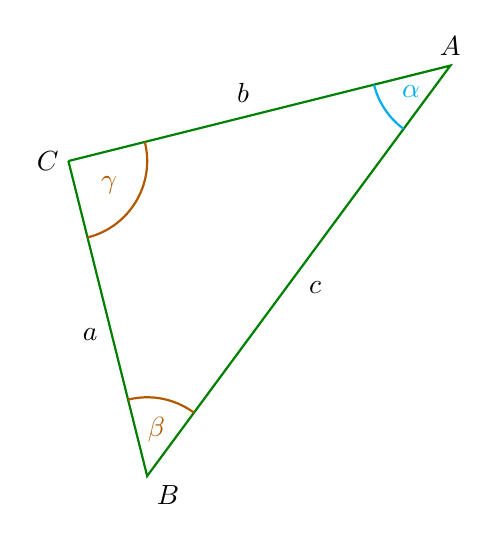
\begin{tikzpicture}[scale=1]
			\RectTri{(0,4)}{(1,0)}{5cm}
			\end{tikzpicture}
			\caption{ត្រីកោណនៃទ្រឹស្តីបទកូសុីនុស និងសុីនុស}
		\end{figure}
	\end{multicols}
\end{theorem}
\section{ផលគុណស្កាលែនៃពីរវុិចទ័រ}
	\begin{multicols}{2}
	\emph{\kml ផលគុណស្កាលែនៃពីរវុិចទ័រៈ} បើគេមានវុិចទ័រពីរ $\overrightarrow{A}$ និង $\overrightarrow{B}$ ដែលផ្គុំគ្នាបានមុំ $\theta$ ដូចរូបខាងស្តាំ។ \newline
	នោះគេអាចសរសេរ
		\begin{align*}
			\text{គេសរសេរ}\quad :&\quad\overrightarrow{A}\cdot\overrightarrow{B}=\abs{\overrightarrow{A}}\abs{\overrightarrow{B}}\cos\theta\\
			\text{ម្យ៉ាងទៀត}\quad :&\quad \quad\overrightarrow{A}\cdot\overrightarrow{B}=AB\cos\theta\\
			\text{បើ}\quad :&\quad\overrightarrow{A}\cdot\overrightarrow{B}=0 \quad \text{នោះ}\quad \overrightarrow{A}\perp\overrightarrow{B}\\
			\text{ដែល}\quad :&\quad  \abs{\overrightarrow{A}}=A\quad \text{និង}\quad \abs{\overrightarrow{B}}=B\quad \text{ហៅថាណម ឬប្រវែងនៃវុិចទ័រ}
		\end{align*}
		\begin{figure}[H]
			\centering
			\begin{tikzpicture}[scale=1.3]
			\begin{scope}
			\coordinate (O) at (0,0);
			\coordinate (A) at (2,2);
			\coordinate (B) at (3,0);
			\coordinate (C) at (4,2);
			\draw [->] (O) -- (A);
			\draw [->] (O) -- (B);
			\draw [dashed] (A) -- (2,0);
			\coordinate[label=above:$\overrightarrow{A}$] (A) at (A);
			\coordinate[label=below:$\overrightarrow{B}$] (B) at (B);
			\pic [draw, -, "$\theta$", angle eccentricity=1.5] {angle = B--O--A};
			\end{scope}
			\end{tikzpicture}
			\caption{ផលគុណស្កាលែនៃពីរវុិចទ័រ}
		\end{figure}
	\end{multicols}
\section{ធរណីមាត្រក្នុងប្លង់ និងអនុគមន៍ត្រីកោណមាត្រ}
\subsection{ការេ}
គេមានការេ $ABCD$ ដែលមានជ្រុង $a$ ដូចរូប។ គេបាន
\begin{multicols}{2}
	\begin{align*}
		\text{ជ្រុង}\quad :&\quad \abs{AB}=\abs{BC}=\abs{CD}=\abs{DA}=a\\
		\text{អង្កត់ទ្រូង}\quad :&\quad \abs{AC}=\abs{BD}=a\sqrt{2}\\
		\text{ពីកំពូលទៅផ្ចិត}\quad :&\quad \abs{AO}=\abs{BO}=\abs{CO}=\abs{DO}=\frac{a\sqrt{2}}{2}\\
		\text{បរិមាត្រ}\quad :&\quad P=4a\\
		\text{ផ្ទៃក្រឡា}\quad :&\quad S=a\cdot a=a^{2}
	\end{align*}
	\begin{figure}[H]
		\centering
		\begin{tikzpicture}
			\begin{scope}
				\coordinate[label=below left:$A$] (A) at (0,0);
				\coordinate[label=below right:$B$] (B) at (3,0);
				\coordinate[label=above right:$C$] (C) at (3,3);
				\coordinate[label=above left:$D$] (D) at (0,3);
				\coordinate[label=below:$O$] (O) at (1.5,1.5);
				\coordinate[label=above:$a$] (a) at (1.5,3);
				\draw (A)--(B)--(C)--(D)--cycle;
				\draw[dashed] (A)--(C);
				\draw[dashed] (B)--(D);
			\end{scope}
		\end{tikzpicture}
		\caption{ការេ}
	\end{figure}
\end{multicols}
\subsection{ចតុកោណកែង}
គេមានចតុកោណកែង $ABCD$ ដែលមានទទឹង​ $a$ និងបណ្តោយ $b$ ដូចរូប។ គេបាន
\begin{multicols}{2}
	\begin{align*}
	\text{ជ្រុង}\quad :&\quad \abs{AD}=\abs{BC}=a,~\abs{AB}=\abs{DC}=b\\
	\text{អង្កត់ទ្រូង}\quad :&\quad \abs{AC}=\abs{BD}=\sqrt{a^{2}+b^{2}}\\
	\text{បរិមាត្រ}\quad :&\quad P=2a+2b\\
	\text{ផ្ទៃក្រឡា}\quad :&\quad S=a\cdot b
	\end{align*}
	\begin{figure}[H]
		\centering
		\begin{tikzpicture}
		\begin{scope}
		\coordinate[label=below left:$A$] (A) at (0,0);
		\coordinate[label=below right:$B$] (B) at (4,0);
		\coordinate[label=above right:$C$] (C) at (4,3);
		\coordinate[label=above left:$D$] (D) at (0,3);
		\coordinate[label=below:$O$] (O) at (2,1.5);
		\coordinate[label=above:$b$] (b) at (2,3);
		\coordinate[label=right:$a$] (a) at (4,1.5);
		\draw (A)--(B)--(C)--(D)--cycle;
		\draw[dashed] (A)--(C);
		\draw[dashed] (B)--(D);
		\end{scope}
		\end{tikzpicture}
		\caption{ចតុកោណកែង}
	\end{figure}
\end{multicols}
\subsection{ប្រភេទនៃត្រីកោណ}
\begin{enumerate}[m]
	\item \emph{\kml ត្រីកោណសាមញ្ញ}
	\begin{multicols}{2}
		គេមានត្រីកោណ $ABC$ ដែលមានកម្ពស់ $h$ ដូចរូប។
		\begin{align*}
		\text{យើងបាន}\quad :&\quad \text{ផ្ទៃក្រឡា}=\frac{\text{បាត}\times \text{កម្ពស់}}{2}\\
		\text{គេអាចសរសេរ}\quad :&\quad S=\frac{AC\times h}{2}\\
		\text{មុំ}\quad :&\quad \alpha + \beta + \theta =180^\circ
		\end{align*}
			\begin{figure}[H]
			\centering
			\begin{tikzpicture}
			\begin{scope}
				\coordinate[label=below left:$A$] (A) at (-1,0);
				\coordinate[label=above right:$B$] (B) at (4,3);
				\coordinate[label=below right:$C$] (C) at (6,0);
				\coordinate[label=below:$H$] (H) at (4,0);
				\coordinate[label=right:$h$] (h) at (4,1.5);
				\draw (A)--(B)--(C)--cycle;
				\draw (B)--(H);
			\end{scope}
			\end{tikzpicture}
			\caption{ត្រីកោណសាមញ្ញ}
		\end{figure}
	\end{multicols}
	\item \emph{\kml ត្រីកោណកែង} គេមានត្រីកោណកែង $ABC$ ដែលមានកម្ពស់ $h$ ដូចរូប។
	\begin{multicols}{2}
		\begin{align*}
			\text{យើងបានក្រឡាផ្ទៃ}\quad :&\quad  S=\frac{AC\times h}{2}\\
			\text{មុំ}\quad :&\quad \alpha + \beta + \theta =180^\circ\\
			\text{ដែល}\quad :&\quad \theta = 90^\circ
		\end{align*}
		\begin{figure}[H]
			\centering
			\begin{tikzpicture}
				\begin{scope}
					\coordinate[label=below left:$A$] (A) at (-1,0);
					\coordinate[label=above right:$B$] (B) at (4,3);
					\coordinate[label=below right:$C$] (C) at (4,0);
%					\coordinate[label=below:$H$] (H) at (4,0);
					\coordinate[label=right:$h$] (h) at (4,1.5);
					\draw (A)--(B)--(C)--cycle;
%					\draw (B)--(H);
				\end{scope}
			\end{tikzpicture}
			\caption{ត្រីកោណកែង}
		\end{figure}
	\end{multicols}
	\item \emph{\kml ត្រីកោណសមបាត} គេមានត្រីកោណសមបាត $ABC$ ដូចរូប។ យើងបាន
	\begin{multicols}{2}
		\begin{align*}
			\text{ជ្រុង}\quad :&\quad \abs{AB}=\abs{BC}=\abs{AC}\times\frac{\sqrt{2}}{2}\\
			\text{កម្ពស់}\quad :&\quad \abs{BH}=\abs{AH}=\abs{HC}=\frac{AC}{2}\\
			\text{មុំ}\quad :&\quad \alpha + \beta + \theta =180^\circ\\
			\text{ដែល}\quad :&\quad \theta = \beta = 45^\circ
		\end{align*}
		\begin{figure}[H]
			\centering
			\begin{tikzpicture}
				\begin{scope}
				\coordinate[label=below left:$A$] (A) at (0,0);
				\coordinate[label=above right:$B$] (B) at (3,3);
				\coordinate[label=below right:$C$] (C) at (6,0);
				\coordinate[label=below:$H$] (H) at (3,0);
				\coordinate[label=right:$h$] (h) at (3,1.5);
				\draw (A)--(B)--(C)--cycle;
				\draw (B) -- (H);
				\end{scope}
			\end{tikzpicture}
			\caption{ត្រីកោណសមបាត}
		\end{figure}
	\end{multicols}
	\item \emph{\kml ត្រីកោណសម័ង្ស} គេមានត្រីកោណសម័ង្ស $ABC$ ដូចរូប។ យើងបានៈ
		\begin{multicols}{2}
			\begin{align*}
			\text{ជ្រុង}\quad :&\quad \abs{AB}=\abs{BC}=\abs{AC}=a\\
			\text{កម្ពស់}\quad :&\quad \abs{BH}=\frac{a\sqrt{3}}{2}\\
			\text{មុំ}\quad :&\quad \alpha + \beta + \theta =180^\circ\\
			\text{ដែល}\quad :&\quad \theta = \beta = \alpha=60^\circ
			\end{align*}
			\begin{figure}[H]
				\centering
				\begin{tikzpicture}
				\begin{scope}
				\coordinate[label=below left:$A$] (A) at (0,0);
				\coordinate[label=above right:$B$] (B) at (2,4);
				\coordinate[label=below right:$C$] (C) at (4,0);
				\coordinate[label=below:$H$] (H) at (2,0);
				\coordinate[label=right:$h$] (h) at (2,1.5);
				\coordinate[label=right:$a$] (a) at (3.3,1.5);
				\draw (A)--(B)--(C)--cycle;
				\draw (B) -- (H);
				\end{scope}
				\end{tikzpicture}
				\caption{ត្រីកោណសមបាត}
			\end{figure}
		\end{multicols}
\end{enumerate}
	\chapter{ទំហំវុិចទ័រ និងទំហំស្កាលែ}
\section{ទំហំវុិចទ័រ}
\subsection{ទំហំវិុចទ័រ}
\quad នៅក្នុងរូបវិទ្យា គេចែកទំហំជាពីរគឺ \emph{ទំហំស្កាលែ និងទំហំវុិចទ័រ}។
\begin{definition}
	\emph{{\kml ទំហំវិុចទ័រៈ}} ជាទំហំដែលសំដែងដោយចំនួនពីជគណិត ហើយបញ្ជាក់ពី ទិស ទិសដៅ។ វុិចទ័រមួយជាអង្គត់ដែលមានទិសដៅ ភ្ជាប់ពីរចំណុចផ្សេងគ្នា ដែលចំណុចំណុចមួយជាគល់ ឬចំណុចចាប់ និងមួយទៀតជាចុងនៃវុិចទ័រ។\\
	\emph{\kml ឧទាហរណ៍ៈ} មនុស្សម្នាក់ជិះកង់ពីទិសខាងលិចទៅខាងកើតដោយល្បឿន $v=10.8km/h$។ 
\end{definition}
\begin{example}
	ទំហំវិុចទ័ររួមមានៈ កម្លាំង ល្បឿន សំទុះទំនាញដី ដែនម៉ាញេទិច។ ល។ យើងអាចលើកយកវុិចទ័រ $\overrightarrow{OA}$ មកសិក្សាៈ
	\begin{multicols}{2}
		\begin{itemize}
			\item [$-$] ចំណុចចាប់ ឬគល់ៈ ត្រង់ $O$
			\item [$-$] ទិសៈ ស្ថិតលើបន្ទាត់ $OA$
			\item [$-$] ទិសដៅពី $O$ ទៅ $A$(សម្គាល់ដោយព្រួញ)
			\item [$-$] អាំងតង់សុីតេ ឬម៉ូឌុលៈ $\abs{\overrightarrow{OA}}$
		\end{itemize}
		\begin{figure}[H]
			\centering
			\begin{tikzpicture}[scale=1]
				\begin{scope}
					\coordinate (O) at (0,0);
					\coordinate (A) at (3,2);
					\draw [->] (O) -- (A);
					\coordinate [label=below:$O$] (O) at (O);
					\coordinate [label=above:$A$] (A) at (A);
					\draw (O) node {$\bullet$};
					\draw (1.2,1.5) node {$\overrightarrow{OA}$};
				\end{scope}
			\end{tikzpicture}
			\caption{វុិចទ័រ}
		\end{figure}
	\end{multicols}
\end{example}
\subsection{វុិចទ័រពីរស្មើគ្នា}
\begin{definition}
	\emph{{\kml វុិចទ័រពីរស្មើគ្នាៈ}} កាលណាវុិចទ័រទាំងពីរនោះមានប្រវែងស្មើគ្នា និងមានទិសដៅដូចគ្នា។
\end{definition}
\begin{example}
	ចូរពិនិត្យមើលវិុចទ័រ $\overrightarrow{A}$ និង $\overrightarrow{B}$ ដូចរូបខាងក្រោម។ យើងឃើញថាវុិចទ័រទាំងពីរនេះមានម៉ូឌុល ឬប្រវែងស្មើគ្នា និងមានទិសដៅដូចគ្នា។
	\begin{figure}[H]
		\centering
		\begin{tikzpicture}
			\begin{scope}
				\draw[->] (.1,-.8) --(6,-.8);
				\draw[->] (.5,-1.2) --(.5,2.5);
				\coordinate (O) at (0,0);
				\coordinate (A) at (3,2);
				\coordinate (B) at (2,0);
				\coordinate (C) at (5,2);
				\draw [->] (O) -- (A);
				\draw [->] (B) -- (C);
				\draw (1.2,1.5) node {$\overrightarrow{A}$};
				\draw (3.2,1.5) node {$\overrightarrow{B}$};
				\coordinate [label=below:$O$] (O) at (0.2,-.8);
				\coordinate [label=left:$y$] (y) at (0.5,2.2);
				\coordinate [label=below:$x$] (x) at (6,-.8);
			\end{scope}
		\end{tikzpicture}
		\caption{វុិចទ័រពីរស្មើគ្នា}
	\end{figure}
	ដូចនេះ វុិចទ័រ $\overrightarrow{A}$ ស្មើនឹង $\overrightarrow{B}$ ឬវុិចទ័រទាំងពីរនេះសមភាពគ្នា ទោះបីវាចេញពីគល់ផ្សេងគ្នាក៏ដោយ។ 
	\begin{align*}
		\text{គេសរសេរៈ}\quad :&\quad \overrightarrow{A}=\overrightarrow{B}\\
		\text{នាំឲ្យ}​\quad :&\quad \abs{\overrightarrow{A}}=\abs{\overrightarrow{B}}\quad \text{ឬ}\quad A=B
	\end{align*}
\end{example}
\subsection{ផលបូកវុិចទ័រ}
\begin{enumerate}[m]
	\item \emph{\kml ផលបូកវុិចទ័រពីរមានទិស និងទិសដៅដូចគ្នា}
	\begin{multicols}{2}
			\quad គេមានវុិចទ័រពីរ $\overrightarrow{A}$ និង $\overrightarrow{B}$ ដូចរូបខាងស្តាំ។\\
		យើងបានវិុចទ័រផ្គួបនៃវុិចទ័រ $\overrightarrow{A}$ និង $\overrightarrow{B}$ គឺ $\fbox{$\overrightarrow{C}=\overrightarrow{A}+\overrightarrow{B}$}$
		\begin{figure}[H]
			\centering
			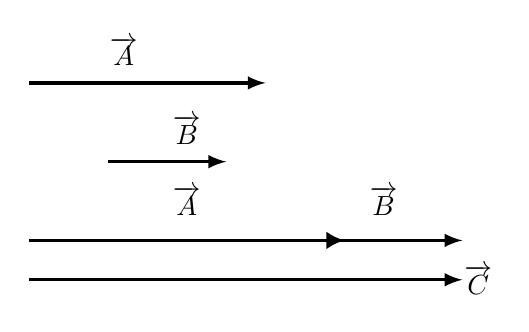
\begin{tikzpicture}
			\begin{scope}[very thick, every node/.style={sloped,allow upside down}]
			\coordinate (O) at (0,2);
			\coordinate (A) at (3,2);
			\coordinate (B) at (1,1);
			\coordinate (C) at (2.5,1);
			\coordinate (D) at (5.5,0);
			\draw [->] (O) -- (A);
			\draw [->] (B) -- (C);
			\draw [->] (0,0) -- (D);
			\draw [arrows = {-Latex[width=6.5pt, length=6.5pt]}] (3.8,0) -- (4,0);
			\draw (1.2,2.4) node {$\overrightarrow{A}$};
			\draw (2,1.4) node {$\overrightarrow{B}$};
			\draw (2,.5) node {$\overrightarrow{A}$};
			\draw (4.5,.5) node {$\overrightarrow{B}$};
			\draw [->] (0,-.5) -- (5.5,-.5);
			\draw (5.7,-.5) node {$\overrightarrow{C}$};
			\end{scope}
			\end{tikzpicture}
			\caption{ផលបូកវុិចទ័រពីរមានទិស និងទិសដៅដូចគ្នា}
		\end{figure}
	\end{multicols}
	ក្នុងករណីដែលយើងចង់រកម៉ូឌុលនៃវុិច $\overrightarrow{C}$ យើងត្រូវលើកអង្គទាំងពីរជាការេ
	\begin{align*}
		\text{យើងបាន}\quad :&\quad \overrightarrow{C^{2}} =\left(\overrightarrow{A}+\overrightarrow{B}\right)^{2}=\overrightarrow{A^{2}} + 2\overrightarrow{A}\overrightarrow{B}+\overrightarrow{B^{2}}=\overrightarrow{A^{2}} + 2AB\cos\left(\overrightarrow{A},\overrightarrow{B}\right) +\overrightarrow{B^{2}}\\
		\text{ដោយ}\quad :&\quad \overrightarrow{C^{2}}=C^{2},~\overrightarrow{A^{2}}=A^{2},~\overrightarrow{B^{2}}=B^{2},~\left(\overrightarrow{A},\overrightarrow{B}\right)=0\\
		\text{យើងបាន}\quad :&\quad C^{2}=A^{2}+2AB+B^{2}=\left(A+B\right)^{2}\\
		\text{នាំឲ្យ}\quad :&\quad C=\sqrt{\left(A+B\right)^{2}}=A+B
	\end{align*}
	\begin{generality}
		អាំងតង់សុីតេវុិចទ័រផ្គួបដែលមានទិសស្របគ្នា និងទិសដៅដូចគ្នាស្មើនឹងផលបូកអាំងតង់សុីតេនៃវុិចទ័រផ្គុំទាំងអស់។
	\end{generality}
	\item \emph{\kml ផលបូកវុិចទ័រពីរមានទិសដូចគ្នា និងទិសដៅផ្ទុយគ្នា}
	\begin{multicols}{2}
		គេមានវុិចទ័រពីរ $\overrightarrow{A}$ និង $\overrightarrow{B}$ ដូចរូបខាងស្តាំ។ គេបានវុិចទ័រ $\overrightarrow{C}=\overrightarrow{A}+\left(-\overrightarrow{B}\right)=\overrightarrow{A}-\overrightarrow{B}\Rightarrow\fbox{$C=A-B$}$\\
		\begin{figure}[H]
			\centering
			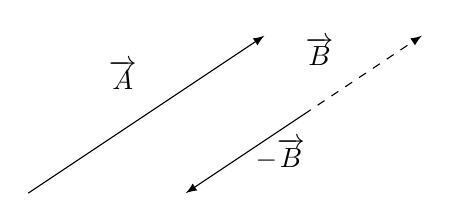
\begin{tikzpicture}
			\begin{scope}
			\coordinate (O) at (0,0);
			\coordinate (A) at (3,2);
			\coordinate (B) at (2,0);
			\coordinate (C) at (3.5,1);
			\coordinate (D) at (3.5,1);
			\coordinate (E) at (5,2);
			\draw [->] (O) -- (A);
			\draw [<-] (B) -- (C);
			\draw[->, dashed] (D) -- (E);
			\draw (1.2,1.5) node {$\overrightarrow{A}$};
			\draw (3.7,1.8) node {$\overrightarrow{B}$};
			\draw (3.2,.5) node {$-\overrightarrow{B}$};
			\end{scope}
			\end{tikzpicture}
			\caption{\koc វុិចទ័រពីរមានទិសដូចគ្នា និងទិសដៅផ្ទុយគ្នា}
		\end{figure}
	\end{multicols}
	\begin{multicols}{2}
		ដើម្បីសង់វុិចទ័រផ្គួប $\overrightarrow{C}$ យើងរំកិលវុិចទ័រ $\overrightarrow{B}$ ដោយរក្សាទិសរបស់វាទៅដាក់លើទិសនៃវុិចទ័រ $\overrightarrow{A}$ ដោយដាក់គល់នៃវុិចទ័រ $\overrightarrow{B}$ លើចុងស្លាបព្រួញនៃវុិចទ័រ $\overrightarrow{A}$។
		\begin{figure}[H]
			\centering
			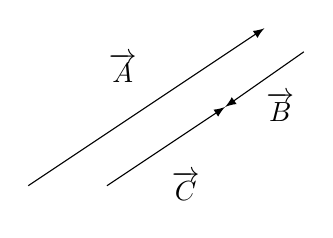
\begin{tikzpicture}
			\begin{scope}
			\coordinate (O) at (0,0);
			\coordinate (A) at (3,2);
			\coordinate (B) at (1,0);
			\coordinate (C) at (2.5,1);
			\coordinate (D) at (2.5,1);
			\coordinate (E) at (3.5,1.7);
			\draw [->] (O) -- (A);
			\draw [->] (B) -- (C);
			\draw[<-] (D) -- (E);
			\draw (1.2,1.5) node {$\overrightarrow{A}$};
			\draw (3.2,1) node {$\overrightarrow{B}$};
			\draw (2,0) node {$\overrightarrow{C}$};
			\end{scope}
			\end{tikzpicture}
			\caption{\koc ផលបូកវុិចទ័រពីរមានទិសដូចគ្នា និងទិសដៅផ្ទុយគ្នា}
		\end{figure}
	\end{multicols}	
	\begin{remark}
		ទិសដៅនៃវុិចទ័រផ្គួបគឺដូចនឹងទិសដៅនៃវុិចទ័រដែលមានអាំងតង់សុីតេធំជាងគេ។
	\end{remark}
	\item \emph{\kml ផលបូកវុិចទ័រពីរមានទិសបង្កើតបានមុំ $\theta$}
		\begin{multicols}{2}
			\quad គេមានវុិចទ័រពីរ $\overrightarrow{A}$ និង $\overrightarrow{B}$ ដែលផ្គុំគ្នាបានមុំ $\theta$ ដូចរូបខាងស្តាំ។ យើងបានវុិចទ័រផ្គួបនៃវុិចទ័រ $\overrightarrow{A}$ និង $\overrightarrow{B}$ គឺតាងដោយ $\overrightarrow{C}=\overrightarrow{A}+\overrightarrow{B}$
			\begin{figure}[H]
				\centering
				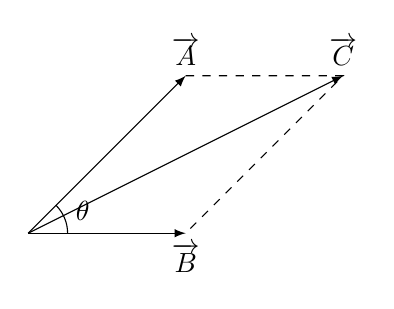
\begin{tikzpicture}
				\begin{scope}
				\coordinate (O) at (0,0);
				\coordinate (A) at (2,2);
				\coordinate (B) at (2,0);
				\coordinate (C) at (4,2);
				\draw [->] (O) -- (A);
				\draw [->] (O) -- (B);
				\draw [->] (O) -- (C);
				\draw [dashed] (2,2) --(4,2) -- (2,0);
				\coordinate[label=above:$\overrightarrow{A}$] (A) at (A);
				\coordinate[label=below:$\overrightarrow{B}$] (B) at (B);
				\coordinate[label=above:$\overrightarrow{C}$] (C) at (C);
				\pic [draw, -, "$\theta$", angle eccentricity=1.5] {angle = B--O--A};
				\end{scope}
				\end{tikzpicture}
				\caption{\koc ផលបូកវុិចទ័រពីរមានទិសបង្កើតបានមុំ $\theta$}
			\end{figure}
		\end{multicols}
		យើងអាចលើកអង្គទាំងពីរនៃសមីការនេះជាការេ
		\begin{align*}
		\text{យើងបាន}\quad :&\quad \overrightarrow{C^{2}} =\left(\overrightarrow{A}+\overrightarrow{B}\right)^{2}=\overrightarrow{A^{2}} + 2\overrightarrow{A}\overrightarrow{B}+\overrightarrow{B^{2}}=\overrightarrow{A^{2}} + 2AB\cos\left(\overrightarrow{A},\overrightarrow{B}\right) +\overrightarrow{B^{2}}\\
		\text{ដោយ}\quad :&\quad \overrightarrow{C^{2}}=C^{2},~\overrightarrow{A^{2}}=A^{2},~\overrightarrow{B^{2}}=B^{2},~\left(\overrightarrow{A},\overrightarrow{B}\right)=\theta\\
		\text{យើងបាន}\quad :&\quad C^{2}=A^{2}+B^{2} + 2AB\cos\theta\\
		\text{នាំឲ្យ}\quad :&\quad C=\sqrt{A^{2}+B^{2}+2AB\cos\theta}
		\end{align*}
	\begin{remark}
		ដើម្បីសង់វុិចទ័រផ្គួប $\overrightarrow{C}$ ដែល $\overrightarrow{C}=\overrightarrow{A}+\overrightarrow{B}$ យើងត្រូវអនុវត្តតាមវិធានអង្តត់ទ្រូងប្រលេឡូក្រាម។
	\end{remark}
	\item \emph{\kml ផលបូកវុិចទ័រពីរមានទិស និងទិសដៅកែងគ្នា}
	\begin{multicols}{2}
		\quad គេមានវុិចទ័រពីរ $\overrightarrow{A}$ និង $\overrightarrow{B}$ ដែលផ្គុំគ្នាបានមុំ $90^\circ$ ឬមានទិស និងទិសដៅកែងគ្នា ដូចរូបខាងស្តាំ។ យើងបានវុិចទ័រផ្គួបនៃវុិចទ័រ $\overrightarrow{A}$ និង $\overrightarrow{B}$ គឺតាងដោយ $\overrightarrow{C}=\overrightarrow{A}+\overrightarrow{B}$
		\begin{figure}[H]
			\centering
			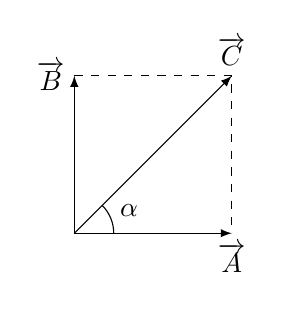
\begin{tikzpicture}
			\begin{scope}
			\coordinate (O) at (0,0);
			\coordinate (A) at (2,0);
			\coordinate (B) at (0,2);
			\coordinate (C) at (2,2);
			\draw [->] (O) -- (A);
			\draw [->] (O) -- (B);
			\draw [->] (O) -- (C);
			\draw [dashed] (0,2) --(2,2) -- (2,0);
			\coordinate[label=below:$\overrightarrow{A}$] (A) at (A);
			\coordinate[label=left:$\overrightarrow{B}$] (B) at (B);
			\coordinate[label=above:$\overrightarrow{C}$] (C) at (C);
			\pic [draw, -, "$\alpha$", angle eccentricity=1.5] {angle = A--O--C};
			\end{scope}
			\end{tikzpicture}
			\caption{\koc ផលបូកវុិចទ័រពីរមានទិស និងទិសដៅកែងគ្នា}
		\end{figure}
	\end{multicols}
	យើងអាចលើកអង្គទាំងពីរនៃសមីការនេះជាការេ
	\begin{align*}
		\text{យើងបាន}\quad :&\quad \overrightarrow{C^{2}} =\left(\overrightarrow{A}+\overrightarrow{B}\right)^{2}=\overrightarrow{A^{2}} + 2\overrightarrow{A}\overrightarrow{B}+\overrightarrow{B^{2}}=\overrightarrow{A^{2}} + 2AB\cos\left(\overrightarrow{A},\overrightarrow{B}\right) +\overrightarrow{B^{2}}\\
		\text{ដោយ}\quad :&\quad \overrightarrow{C^{2}}=C^{2},~\overrightarrow{A^{2}}=A^{2},~\overrightarrow{B^{2}}=B^{2},~\left(\overrightarrow{A},\overrightarrow{B}\right)=90^\circ\\
		\text{យើងបាន}\quad :&\quad C^{2}=A^{2}+B^{2}\\
		\text{នាំឲ្យ}\quad :&\quad C=\sqrt{A^{2}+B^{2}}
	\end{align*}
\end{enumerate}
\section{ទំហំស្កាលែ}
\begin{definition}
	\emph{\kml ទំហំស្កាលែៈ} ជាទំហំដែលសំដែងដោយចំនួនពីជគណិត មិនគិតពី ទិស ទិសដៅឡើយ។ នៅក្នុងរូបវិទ្យាទំហំដែលមិនទាក់ទងនឹងទិសដៅ(ទំហំស្កាលែ) មានដូចជាៈ សីតុណ្ហភាព សម្ពាធ ថាមពល កម្មន្ត ម៉ាស រយៈពេល។ ល។\\
	\emph{\kml ឧទាហរណ៍ៈ} កីឡាករម្នាក់រត់បានចម្ងាយ $100m$ ដោយប្រើរយៈពេល $10s$។\\ ចម្ងាយ $100m$ និងរយៈពេល $10s$ ជាទំហំស្កាលែ។
\end{definition}
\section{កូអរដោនេនៃវិុចទ័រ}
	\begin{multicols}{2}
		ឧបមាថាយើងមានត្រីកោណកែង $ABC$ ដូចបង្ហាញក្នុងរូបខាងស្តាំ ។
		\begin{equation*}
			\sin\theta=\frac{\text{ជ្រុងឈម}}{\text{អុីប៉ូតេនុស}},\quad \cos\theta=\frac{\text{ជ្រុងជាប់}}{\text{អុីប៉ូតេនុស}},\quad \tan\theta=\frac{\text{ជ្រុងឈម}}{\text{ជ្រុងជាប់}}
		\end{equation*}
		\begin{figure}[H]
			\centering
			\begin{tikzpicture}
				\centering 
				\begin{scope}
				\large
				\coordinate (C) at (0,0);
				\coordinate (A) at (3,0);
				\coordinate (B) at (3,2);
				\draw (C) -- (A) -- (B) -- cycle;
				\pic [draw, -, "$\theta$", angle eccentricity=1.5] {angle = A--C--B};
				\draw (A) -- ++ (0, .3cm) -- ++ (-.3cm, 0) -- ++ (0, -.3cm);
				\coordinate[label=below:$A$] (A) at (A);
				\coordinate[label=above:$B$] (B) at (B);
				\coordinate[label=below:$C$] (C) at (C);
				\coordinate[label=below:{\text{ជ្រុងជាប់}}] (1.5,0) at (1.5,0);
				\coordinate[label=right:{\text{ជ្រុងឈម}}] (3,1) at (3,1);
				\coordinate[label=right:{\text{អុីប៉ូតេនុស}}] (-1,1) at (-1,1);
				\end{scope}
			\end{tikzpicture}
			\caption{\koc ទំនាក់ទំនងក្នុងត្រីកោណមាត្រ}
		\end{figure}
	\end{multicols}
	ទំនាក់ទំនង់រវាង $\sin\theta$ និង $\cos\theta$ គឺ
	\begin{align*}
		\tan\theta=\frac{\sin\theta}{\cos\theta} \quad \text{និង}\quad \sin^{2}\theta+\cos^{2}\theta=1
	\end{align*}
	\begin{multicols}{2}
		គេមានវុិចទ័រ $\overrightarrow{A}$ ស្តិតក្នុងប្លង់ $xy$ និងបង្កើតបានមុំ $\theta$ ជាមួយអ័ក្ស $Ox$ ដូចរូប។\\ យើងចំណោលកែងវុិចទ័រ $\overrightarrow{A}$ លើអ័ក្ស $Ox$ និង $Oy$ យើងបានធាតុរបស់វា{\en(Components of Vectors)}គឺ $\overrightarrow{A_{x}}$ និង $\overrightarrow{A_{y}}$។ តាមលក្ខណៈនៃវុិចទ័រយើងបានៈ $\overrightarrow{A}=\overrightarrow{A_{x}}+\overrightarrow{A_{y}}$
		\begin{figure}[H]
			\centering
			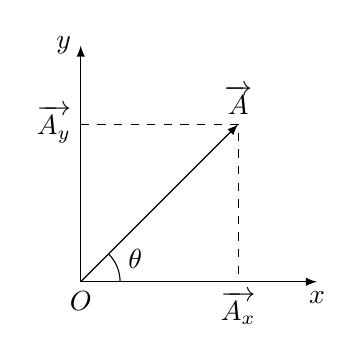
\begin{tikzpicture}
			\begin{scope}
			\coordinate (O) at (0,0);
			\coordinate (x) at (3,0);
			\coordinate (y) at (0,3);
			\coordinate (A) at (2,2);
			\draw [->] (O) -- (x);
			\draw [->] (O) -- (y);
			\draw [->] (O) -- (A);
			\draw [dashed] (0,2) --(2,2) -- (2,0);
			\coordinate[label=below:$x$] (x) at (x);
			\coordinate[label=left:$y$] (y) at (y);
			\coordinate[label=above:$\overrightarrow{A}$] (A) at (A);
			\coordinate[label=below:$\overrightarrow{A_{x}}$] (2,0) at (2,0);
			\coordinate[label=left:$\overrightarrow{A_{y}}$] (0,2) at (0,2);
			\coordinate[label=below:$O$] (0,0) at (0,0);
			\pic [draw, -, "$\theta$", angle eccentricity=1.5] {angle = x--O--A};
			\end{scope}
			\end{tikzpicture}
			\caption{\koc ផលបូកវុិចទ័រពីរមានទិស និងទិសដៅកែងគ្នា}
		\end{figure}
	\end{multicols}
	\begin{proof}
		\begin{align*}
			\text{ដែល}\quad :&\quad A_{x}=A\cos\theta \quad\text{និង}\quad A_{y}=A\sin\theta\\
				\text{យើងបាន}\quad :&\quad \overrightarrow{A^{2}} =\left(\overrightarrow{A_{x}}+\overrightarrow{A_{y}}\right)^{2}=\overrightarrow{A^{2}_{x}} + 2\overrightarrow{A_{x}}\overrightarrow{A_{y}}+\overrightarrow{A_{y}^{2}}=\overrightarrow{A៌_{x}^{2}} + 2A_{x}A_{y}\cos\left(\overrightarrow{A_{x}},\overrightarrow{A_{y}}\right) +\overrightarrow{A_{y}^{2}}\\
			\text{ដោយ}\quad :&\quad \overrightarrow{A^{2}}=A^{2},~\overrightarrow{A_{x}^{2}}=A_{x}^{2},~\overrightarrow{A_{y}^{2}}=A_{y}^{2},~\left(\overrightarrow{A_{x}},\overrightarrow{A_{y}}\right)=90^\circ\\
			\text{យើងបាន}\quad :&\quad A^{2}=A_{x}^{2}+A_{y}^{2}\\
			\text{នាំឲ្យ}\quad :&\quad A=\sqrt{A_{x}^{2}+A_{y}^{2}}
		\end{align*}
	\end{proof}
	%\section{លំហាត់}
\begin{enumerate}[m]
	\item ចូរពោលទ្រឹស្តីសុីនេទិចនៃឧស្ម័ន។
	\item ចូរសរសេរសមីការភាពនៃឧស្ម័នបរិសុទ្ធ។
	\item ចូរសរសេររូបមន្តថាមពលសុីនេទិចមធ្យមនៃម៉ូលេគុលឧស្ម័ននីមួយៗ។
	\item ចូរសរសេររូបមន្តថាមពលសុីនេទិចសរុបនៃម៉ូលេគុលឧស្ម័ន។
	\item ចូរសរសេររូបមន្តល្បឿនប្ញសការេនៃការេល្បឿនមធ្យមម៉ូលេគុលឧស្ម័ន។
	\item ក្នុងធុងបិទជិតមួយមានផ្ទុកឧស្ម័នអុកសុីសែន $\left(\ce{O2}\right)~2mol$។\\
	គណនាចំនួនម៉ូលេគុលរបស់ឧស្ម័នអុកសុីសែននេះ បើចំនួនអាវ៉ូកាដ្រូ $N_{A}=6.022\times10^{23}$ ម៉ូលេគុល$/mol$។
	\item ក្នុងធុងបិទជិតមួយមានឧស្ម័នអុីដ្រូសែន $\left(\ce{H2}\right)~0.2mol$ និងមានម៉ាសម៉ូល $2.0g/mol$។\\
	បើគេដឹងថា ចំនួនអាវ៉ូកាដ្រូ $N_{A}=6.022\times10^{23}$ម៉ូលេគុល$/mol$។
	\begin{enumerate}[k]
		\item គណនាចំនួនម៉ូលេគុលអុីដ្រូសែនក្នុងធុងនេះ។
		\item គណនាម៉ាសសរុបរបស់ឧស្ម័នអុីដ្រូសែន។
	\end{enumerate}
	\item ក្នុងធុងបិទជិតមួយមានឧស្ម័ន $0.25mol$ និងមានម៉ាសសរុប $7.0g$។\\
	បើគេដឹងថា ចំនួនអាវ៉ូកាដ្រូ $N_{A}=6.022\times10^{23}$ម៉ូលេគុល$/mol$។
	\begin{enumerate}[k]
		\item គណនាចំនួនម៉ូលេគុលសរុបរបស់ឧស្ម័នក្នុងធុងនេះ។
		\item តើឧស្ម័ននេះជាឧស្ម័នអ្វី?
	\end{enumerate}
	\item ក្នុងធុងបិទជិតមួយមានឧស្ម័នពេញ មានម៉ាសសរុប $64.0g$ និងមានចំនួនម៉ូលេគុលសរុបគឺ $12.044\times10^{23}$ម៉ូលេគុល។\\
	បើគេដឹងថា ចំនួនអាវ៉ូកាដ្រូ $N_{A}=6.022\times10^{23}$ម៉ូលេគុល$/mol$។
	\begin{enumerate}[k]
		\item គណនាចំនួនម៉ូលរបស់ឧស្ម័នក្នុងធុងនេះ។
		\item តើឧស្ម័ននេះជាឧស្ម័នអ្វី?
	\end{enumerate}
	\item ក្នុងធុងបិទជិតមួយមានផ្ទុក ឧស្ម័ន $\ce{H2}$ ពេញមានម៉ាសសរុប $1.0g$។ ដោយឧស្ម័ននេះមានម៉ាសម៉ូល $2.0g/mol$ និងចំនួនអាវ៉ូកាដ្រូ $N_{A}=6.022\times10^{23}$ម៉ូលេគុល$/mol$។
	\begin{enumerate}[k]
		\item គណនាចំនួនម៉ូលេគុលសរុបរបស់ឧស្ម័នក្នុងធុងនេះ។
		\item គណនាចំនួនម៉ូលរបស់ឧស្ម័ន $\ce{H2}$។
	\end{enumerate}
	\item ផង់នីមួយៗមានម៉ាស $m_{0}$ និងផ្លាស់ទីដោយល្បឿន $v$ តាមបណ្តោយអ័ក្ស $\overrightarrow{ox}$។ គេដឹងថាក្នុងផ្ទៃ $1mm^{2}$ និងក្នុង $1s$ មានផង់ចំនួន $10^{15}$ ទៅទង្គិចនឹងផ្ទៃនោះ។
	ចូររកសម្ពាធរបស់ផង់លើផ្ទៃប៉ះ។\\
	គេឲ្យ $m_{0}=9.1\times10^{-31}kg$ និង $v=8\times10^{7}m/s$។ គេសន្មត ទង្គិចរវាងផង់ និងផ្ទៃប៉ះជាទង្គិចស្ទក់។
	\item គេបាញ់ផង់ឲ្យផ្លាស់ទីតាមបណ្តោយអ័ក្ស $\overrightarrow{ox}$ ដែលកែងនឹងផ្ទៃរបស់អេក្រង់មួយ។ គេដឹងថា ផង់នីមួយៗមានម៉ាស $m_{0}$ និងល្បឿន $v_{0}$។ គេដឹងថាក្នុង $1.25mm^{2}$ ផ្ទៃរបស់អេក្រង់មានផង់ចំនួន $4\times10^{14}$ ទៅទង្គិចរៀងរាល់វិនាទី។ \\គេសន្មតថា ទង្គិចនោះជាទង្គិចស្ទក់។ គណនាល្បឿនរបស់ផង់ដែលផ្លាស់ទីតាមអ័ក្ស $\overrightarrow{ox}$។\\ បើគេដឹងថា សម្ពាធដែលកើតឡើងដោយសារការទង្គិចរបស់ផង់លើផ្ទៃអេក្រង់គឺ $P=3.64\times10^{-3}N/m^{2}\\~m_{0}=9.1\times10^{-31}kg$។
	\item ផង់នីមួយមានម៉ាស $m_{0}$ នឹងផ្លាស់ទីដោយល្បឿន $v$ តាមបណ្តោយអ័ក្ស $\overrightarrow{ox}$។ គេដឹងថាក្នុងផ្ទៃ $2mm^{2}$ និងក្នុងមួយវិនាទីមានផង់ចំនួន $2\times10^{15}$ ទៅទង្គិចនឹងផ្ទៃនោះ។ គេឲ្យៈ $m_{0}=9.1\times10^{-31}kg$ និង $v=5\times10^{7}m/s$។ គេសន្មតថា ទង្គិចរវាងផង់ និងផ្ទៃប៉ះជាទង្គិចស្ទក់។
	\begin{enumerate}[k,2]
		\item គណនាកម្លាំងសរុបដែលផង់មានអំពើលើផ្ទៃប៉ះ។
		\item គណនាសម្ពាធសរុបរបស់ផង់លើផ្ទៃប៉ះ។
	\end{enumerate}
	\item ប្រូតុងមួយមានម៉ាស $m_{p}=1.67\times10^{-27}kg$ ផ្លាស់ទីដោយល្បឿន $v$ តាមបណ្តោយអ័ក្ស $\overrightarrow{ox}$ ក្នុងមាឌមួយមានរាងជាគូបដែលទ្រនុងនីមួយៗមានរង្វាស់ $3mm$ ប្រូតុងផ្លាស់ពីផ្ទៃម្ខាងទៀតក្នុង $2ns$។ គេសន្មត់ថា ទង្គិចរវាងប្រូតុង និងផ្ទៃខាងនៃគូបជាទង្គិចស្ទក់។
	\begin{enumerate}[k]
		\item រកល្បឿនដើមប្រូតុង នៅខណៈវាចាប់ផ្តើមចេញពីផ្ទៃខាងនៃគូប។
		\item រកសម្ពាធរបស់ប្រូតុងលើផ្ទៃខាងនៃគូប។
		\item គេដឹងថាក្នុងរយៈពេល $2ns$ មានចំនួនប្រូតុង $2\times10^{6}$ ទៅទង្គិចនឹងផ្ទៃខាងនៃគូប។ រកសម្ពាធសរុបរបស់ប្រូតុងលើផ្ទៃខាងនៃគូប។
	\end{enumerate}
	\item អេឡិចត្រុងមួយមានម៉ាស $m_{e}=9.1\times10^{-31}kg$ ផ្លាស់ទីដោយល្បឿន $v$ តាមបណ្តោយអ័ក្ស $\overrightarrow{ox}$ ក្នុងមាឌមួយមានរាងជាគូបដែលទ្រនុងនីមួយៗមានរង្វាស់ $5mm$ ប្រូតុងផ្លាស់ពីផ្ទៃម្ខាងទៀតក្នុង $25ns$។ \\គេសន្មត់ថា ទង្គិចរវាងប្រូតុង និងផ្ទៃខាងនៃគូបជាទង្គិចស្ទក់។
	\begin{enumerate}[k]
		\item រកល្បឿនដើមអេឡិចត្រុង នៅខណៈវាចាប់ផ្តើមចេញពីផ្ទៃខាងនៃគូប។
		\item រកសម្ពាធរបស់អេឡិចត្រុងលើផ្ទៃខាងនៃគូប។
		\item គេដឹងថាក្នុងរយៈពេល $25ns$ មានចំនួនអេឡិចត្រុង $2\times10^{10}$ ទៅទង្គិចនឹងផ្ទៃខាងនៃគូប។\\ រកសម្ពាធសរុបរបស់អេឡិចត្រុងមានលើផ្ទៃខាងនៃគូប។
	\end{enumerate}
	\item អេឡិចត្រុងមួយមានម៉ាស $m_{e}=9.1\times10^{-31}kg$ ផ្លាស់ទីដោយល្បឿន $v$ តាមបណ្តោយអ័ក្ស $\overrightarrow{ox}$ ក្នុងមាឌមួយមានរាងជាគូបដែលទ្រនុងនីមួយៗមានរង្វាស់ $2mm$ ប្រូតុងផ្លាស់ពីផ្ទៃម្ខាងទៀតក្នុង $25ns$។ គេសន្មត់ថា ទង្គិចរវាងប្រូតុង និងផ្ទៃខាងនៃគូបជាទង្គិចខ្ទាត។
	\begin{enumerate}[k]
		\item រកល្បឿនដើមអេឡិចត្រុង នៅខណៈវាចាប់ផ្តើមចេញពីផ្ទៃខាងនៃគូប។
		\item រកសម្ពាធរបស់អេឡិចត្រុងលើផ្ទៃខាងនៃគូប។
		\item គេដឹងថាក្នុងរយៈពេល $25ns$ មានចំនួនអេឡិចត្រុង $25\times10^{6}$ ទៅទង្គិចនឹងផ្ទៃខាងនៃគូប។\\ រកសម្ពាធសរុបរបស់អេឡិចត្រុងមានលើផ្ទៃខាងនៃគូប។
	\end{enumerate}
	\item អាតូមអុីដ្រូសែនមួយមានម៉ាស $m$ ផ្លាស់ទីដោយល្បឿន $v=1500km/s$ តាមបណ្តោយអ័ក្ស $\overrightarrow{ox}$ ក្នុងមាឌមួយមានរាងគូបដែលទ្រនុងនីមួយមានរង្វាស់ $3mm$។ អុីដ្រូសែន ផ្លាស់ទីពីផ្ទៃម្ខាងទៅម្ខាងទៀត។ គេសន្មតថាសន្មត់ថា ទង្គិចរវាងអុីដ្រូសែន និងផ្ទៃខាងនៃគូបជាទង្គិចខ្នាត។
	\begin{enumerate}[k]
		\item រករយៈពេលដែលអាតូមអុីដ្រូសែនទៅប៉ះនឹងផ្ទៃម្ខាងទៀតនៃគូប។
		\item គេដឹងថាក្នុងរយៈពេល $2ns$ មានចំនួនអាតូមអុីដ្រូសែន $2\times10^{6}$ ទៅទង្គិចនឹងផ្ទៃខាងនៃគូបហើយផ្ទៃខាងរងនៅសម្ពាធសរុប $27.83\times10^{-2}N/m^{2}$។ រកម៉ាសអាតូមអុីដ្រូសែនមួយ។
	\end{enumerate}
	\item ឧស្ម័នបរិសុទ្ធមួយមានមាឌ $V=100cm^{3}$ ស្ថិតក្រោមសម្ពាធ $2.00\times10^{5}Pa$ នៅសីតុណ្ហភាព $20^\circ C$។\\ តើឧស្ម័ននោះមានប៉ុន្មានម៉ូល? $\left(R=8.31J/mol\cdot K\right)$
	\item ឧស្ម័នបរិសុទ្ធមួយមាន $n=0.08\times10^{-1}mol$ មានសម្ពាធ $P=5.00\times10^{5}Pa$ នៅសីតុណ្ហភាព $60^\circ C$។\\ តើឧស្ម័ននោះមានមាឌប៉ុន្មាន?
	\item នៅសីតុណ្ហភាព $293K$ និងសម្ពាធ $5atm$ មេតាន $1kmol$ មានម៉ាស $16.0kg$។ \\គណនាម៉ាសមាឌនៃមេតានក្នុងលក្ខខណ្ឌខាងលើ។
	\item នៅក្នុងបំពង់បិទជិតដែលមានមាឌ $20mL$ នៅសីតុណ្ហភាពកំណត់មួយយ៉ាងទាបមានតំណក់នីត្រូសែនរាវមានម៉ាស $50mg$។ គណនាសម្ពាធនីត្រូសែននៅក្នុងបំពង់នោះ កាលណាបំពង់នោះមានសីតុណ្ហភាព $300K$ ដោយសន្មតថានីត្រូសែននេះជាឧស្ម័នបរិសុទ្ធ។ គេឲ្យៈ $R=8.31J/mol\cdot K$។
	\item ធុងមួយមានផ្ទុកអេល្យូម $2.00mol$ នៅសីតុណ្ហភាព $27^\circ C$។ គេសន្មតថាអេល្យូមជាឧស្ម័នបរិសុទ្ធ។
	\begin{enumerate}[k]
		\item គណនាតម្លៃមធ្យមនៃថាមពលសុីនេទិចរបស់ម៉ូលេគុលនីមួយៗ
		\item គណនាថាមពលសុីនេទិចសរុបរបស់ម៉ូលេគុលទាំងអស់។\\
		គេឲ្យៈ $k_{B}=1.38\times10^{-23}J/K,~R=8.31J/mol\cdot K$។
	\end{enumerate}
	\item នៅក្នុងធុងមួយដែលមានមាឌ $2.00mL$ មានឧស្ម័នដែលមានម៉ាស $50mg$ និងសម្ពាធ $100kPa$។\\ ម៉ាសរបស់មូលេគុលនៃឧស្ម័ននីមួយៗគឺ $8.0\times10^{-26}kg$។
	\begin{enumerate}[k]
		\item រកចំនួនម៉ូលេគុលនៃឧស្ម័ននោះ។
		\item រកតម្លៃមធ្យមនៃថាមពលសុីនេទិចរបស់ម៉ូលេគុលនីមួយៗ។ គេឲ្យៈ $k=1.38\times10^{-23}J/K$
	\end{enumerate}
	\item ចូរគណនាប្ញសការេនៃការេល្បឿនមធ្យមរបស់អាតូមអេល្យូមនៅសីតុណ្ហភាព $20.0^\circ C$។ \\ម៉ាសម៉ូលអេល្យូមគឺ $4.00\times10^{-3}kg/mol$។ គេឲ្យៈ $R=8.31J/mol\cdot K$។
	\item រកប្ញសការេនៃការេល្បឿនមធ្យមរបស់ម៉ូលេគុលអុកសុីសែននៅសីតុណ្ហភាព $200^\circ C$។ \\ម៉ាសម៉ូលអុកសុីសែន $32\times10^{-3}kg/mol$ និង $R=8.31J/mol\cdot K$។
	\item \begin{enumerate}[k]
		\item គណនាម៉ាសម៉ូលេគុលនៃអុីដ្រូសែន។ គេឲ្យម៉ាសម៉ូលគឺ $M=2.00\times10^{-3}kg/mol$ \\និងចំនួនអាវ៉ូកាដ្រូ $N_{A}=6.02\times10^{23}/mol$។
		\item គណនាតម្លៃប្ញសការេនៃការេល្បឿនមធ្យមរបស់ឧស្ម័នអុីដ្រូសែននៅសីតុណ្ហភាព $100^\circ C$។
		\item គណនាតម្លៃមធ្យមនៃថាមពលសុីនេទិចរបស់ម៉ូលេគុលនៃឧស្ម័នអុីដ្រូសែននីមួយៗនៅសីតុណ្ហភាព $100^\circ C$។\\ គេឲ្យៈ $k=1.38\times10^{-23}$។
	\end{enumerate}
	\item ដោយប្រើតម្លៃលេខ $1,3,7$ និង $8$ ចូរបង្ហាញថា ប្ញសការេនៃការេល្បឿនមធ្យម $v_{rms}$ \\ខុសគ្នាពីតម្លៃមធ្យម $v_{av}$ របស់វា។
	\item ចូរកំណត់រកល្បឿន $v_{rms}$ របស់ម៉ូលេគុលឧស្ម័នអុកសុីសែន $\left(O_{2}\right)$ និងអាសូត $\left(N_2\right)$ ក្នុងបន្ទប់មួយដែលមានសីតុណ្ហភាព $20^\circ C$។
	\item \begin{enumerate}[k]
		\item បង្ហាញថាល្បឿន $v_{rms}$ នៃឧស្ម័នបរិសុទ្ធ អាចសរសេរជាទម្រង់មួយទៀតគឺ $v_{rms}=\sqrt{\frac{3P}{\rho}}$ ដែល $\rho$ ជាដង់សុីតេ ឬហៅថាម៉ាសមាឌ ហើយ $P$ ជាសម្ពាធ។
		\item ល្បឿន $v_{rms}$ របស់ម៉ូលេគុលឧស្ម័នមួយប្រភេទស្មើ $450m/s$។\\ ប្រសិនបើវាស្ថិតនៅសម្ពាធបរិយាកាស តើដងសុីតេរបស់ឧស្ម័ននោះស្មើប៉ុន្មាន?
	\end{enumerate}
	\item កែវបាឡុងមួយចំណុះ $1L$ មានអុកសុីសែនជាឧស្ម័នបរិសុទ្ធដែលមានសីតុណ្ហភាព $27^\circ C$ ក្រោមសម្ពាធ $2atm$។\\
	គណនាម៉ាសអុកសុីសែន។ គេឲ្យៈ $O=16$
	\item គេមានខ្យល់មានមាឌ $1m^3$ នៅសីតុណ្ហភាព $18^\circ C$ ក្នុងសម្ពាធបរិយាកាស $P_{1}=1atm$ ទៅបណ្ណែននៅសីតុណ្ហភាពដដែល តែក្នុងសម្ពាធបរិយាកាស $P_{2}=3.5atm$។ គណនាមាឌស្រេចនៃខ្យល់។
	\item ដបមួយផ្ទុកឧស្ម័នមានសម្ពាធ $P_{0}=1.0atm$ នៅសីតុណ្ហភាព $17^\circ C$។\\
	តើគេត្រូវកម្តៅឪ្យឧស្ម័ននេះដល់សីតុណ្ហភាពប៉ុន្មាន ដើម្បីសម្ពាធកើនឡើងដល់ $1.5atm$?
	\item គេយកបំពង់អុកសុីសែនមានចំណុះ $20L$ ក្រោមសម្ពាធ $P_{1}=200atm$ នៅសីតុណ្ហភាព $20^\circ C$ ទៅដាក់ក្នុងបាឡុង កៅស៊ូស្តើងមួយ។ គណនាមាឌបាឡុង បើឧស្ម័នក្នុងបាឡុងមានសម្ពាធ $P_{2}=1atm$ និងសីតុណ្ហភាព $9^\circ C$។
	\item \begin{enumerate}[k]
		\item ចូរគណនាល្បឿនប្រសិទ្ធ $\left(v_{rms}\right)$ នៃម៉ួលេគុលឧស្ម័ននីត្រូសែននៅសីតុណ្ហភាព $20^\circ C$។
		\item គណនាសីតុណ្ហភាព ប្រសិនបើល្បឿនប្រសិទ្ធ $\left(v_{rms}\right)$ ថយចុះពាក់កណ្តាល។
		\item គណនាសីតុណ្ហភាព ប្រសិនបើល្បឿនប្រសិទ្ធ $\left(v_{rms}\right)$ កើនឡើងពីរដងវិញ។
	\end{enumerate}
	\item មួយ ម៉ូលេគុលឧស្ម័ននីដ្រូសែនផ្សំឡើងពីអាតូមនីដ្រូសែនពីរ។គណនាម៉ាសម៉ូលេគុលនីត្រូសែន។\\ ម៉ាសម៉ូលនីដ្រូសែនគឺ $M=28kg/kmol$ គេឲ្យ $N_{A}=6.02\times10^{23}$ ម៉ូលេគុល$/mol$
	\item គណនាមាឌឧស្ម័នអុកសុីសែន $3.2g$ ដែលផ្ទុកក្នុងធុងនៅសម្ពាធ $76cmHg$ និងសីតុណ្ហភាព $27^\circ C$។
	\item រកល្បឿនប្រសិទ្ធ $v_{rms}$ នៃម៉ូលេគុលអាសូតដោយម៉ាសម៉ូល $M=28g/mol$ នៅ $300K$។ គេឲ្យៈ $R=8.31J/mol\cdot K$
	\item គណនាសីតុណ្ហភាពដែលធ្វើឲ្យល្បឿនប្រសិទ្ធនៃម៉ូលេគុលអុីដ្រូសែនស្មើ $331m/s$។ គេឲ្យៈ $M_{H_{2}}=2.0g/mol$។ 
	\item គណនាតម្លៃមធ្យមនៃថាមពលសុីនេទិចនៃម៉ូលេគុលឧស្ម័ននៅសីតុណ្ហភាព $727^\circ C$។ គេឲ្យៈ $R=8.31J/mol\cdot K$ និង $N_{A}=6.02\times10^{23}$ម៉ូលេគុល$/mol$។
	\item រកតម្លៃមធ្យមនៃថាមពលសុីនេទិចរបស់ម៉ូលេគុលឧស្ម័នអុកសុីសែននីមួយៗក្នុងខ្យល់នៅក្នុងបន្ទប់មានសីតុណ្ហភាព $300K$ គិតជាអេឡិចត្រុង-វ៉ុល។ គេឲ្យ $1eV=1.6\times10^{-19}J$ និង $k_{B}=1.38\times10^{-23}J/K$
	\item មួយម៉ូលេគុលនីដ្រូសែននៅពេលស្ថិតនៅលើផ្ទៃដីវាកើតមានល្បឿនប្រសិទ្ធ នៅសីតុណ្ហភាព $0^\circ C$។ ប្រសិនបើវាផ្លាស់ទីឡើងត្រង់ទៅលើដោយគ្មានទង្គិចនឹងម៉ូលេគុលផ្សេងទៀត។ ចូរគណនាកម្ពស់ដែលវាឡើងដល់។ \\គេឲ្យម៉ាសមួយម៉ូលេគុលរបស់នីដ្រូសែន $m=4.65\times10^{-26}kg$ និង $g=10m/s^{2}$។
	\item សុីទែនមួយស្ថិតក្រោមលក្ខខណ្ឌស្តង់ដា {\en (STP)} ផ្ទុកឧស្ម័ននីដ្រូសែន $28.5kg$។
	\begin{enumerate}[k]
		\item ចូរគណនាមាឌរបស់សុីទែន។
		\item ប្រសិនបើគេបន្ថែមនីដ្រូសែន $32.2kg$ ទៀតចូលក្នុងសុីទែនដោយរក្សាសីតុណ្ហភាពនៅដដែល។ \\ចូរគណនាសម្ពាធឧស្ម័ននីដ្រូសែនក្នុងសុីទែន។
	\end{enumerate}
	\item បាច់ម៉ូលេគុលអុីដ្រូសែនត្រូវបានបាញ់លើជញ្ជាំងដោយទិសបង្កើតបានមុំ $55^\circ$ ជាមួយនឹងវុិចទ័រឯកតាផ្ទៃ $\left(\overrightarrow{n}\right)$ របស់ជញ្ជាំង។ ម៉ូលេគុលនីមួយៗនៃឧស្ម័នអុីដ្រូសែនមានល្បឿន $1km/s$ និងម៉ាស $3.3\times10^{-24}kg$។ បាច់អុីដ្រូសែនបានទៅទង្គិចនឹងជញ្ជាំងដែលមានផ្ទៃ $2cm^{2}$ ដោយអត្រា $10^{23}$ ម៉ូលេគុលក្នុងមួយវិនាទី។\\ ដោយសន្មតថាទង្គិចនេះ ជាទង្គិចខ្ទាត ចូរគណនាសម្ពាធដែលមានលើជញ្ជាំង។
	\item គេបាញ់ផង់ឲ្យផ្លាសើទីតាមបណ្តោយអ័ក្ស $\overrightarrow{ox}$ ដែលកែងនឹងផ្ទៃរបស់អេក្រង់មួយ។ គេដឹងថាផង់នីមួយៗមានម៉ាស $m_{0}$ និងមានល្បឿន $v$។ គេដឹងថាក្នុង $1.25mm^{2}$ ផ្ទៃរបស់អេក្រង់មានផង់ $4\times10^{14}$ ទៅទង្គិចរៀងរាល់វិនាទី។\\ គេសន្មត់ថា ទង្គិចនោះជាទង្គិចស្ទក់។
	គណនាល្បឿនរបស់ផង់ដែលផ្លាស់ទីតាមតាមអ័ក្ស $\overrightarrow{ox}$។ បើគេដឹងថា សម្ពាធដែលកើតឡើងដោយសារការទង្គិចរបស់ផង់លើផ្ទៃរបស់អេក្រង់គឺ $3.64\times10^{-3}N\cdot m^{-2}$ និង $m_{0}=9.1\times10^{-31}kg$។
	\item ផង់នីមួយៗមានម៉ាស $m_{0}$ និងផ្លាស់ទីដោយល្បឿន $v$ តាមបណ្តោយអ័ក្ស $\overrightarrow{ox}$។ គេដឹងថាក្នុងផ្ទៃ $2mm^{2}$ និងក្នុងមួយវិនាទីមានផង់ចំនួន $2\times10^{15}$ ទៅទង្គិចនឹងផ្ទៃនោះ។ គេឲ្យៈ $m_{0}=9.1\times10^{-31}kg$ និង $v=5.0\times10^{15}m/s$។\\
	គេសន្មតថា ទង្គិចរវាងផង់និងផ្ទៃប៉ះជាទង្គិចស្ទក់។
	\begin{enumerate}[k]
		\item គណនាកម្លាំងសរុបដែលផង់មានអំពើលើផ្ទៃប៉ះ។
		\item គណនាសម្ពាធសរុបរបស់ផង់លើផ្ទៃប៉ះ។
	\end{enumerate}
	\item  ប្រូតុងមួយមានម៉ាស $m_{P}=1.67\times10^{-27}kg$ និងផ្លាស់ទីដោយល្បឿនដើម $\overrightarrow{v}_{0}$ តាមបណ្តោយអ័ក្ស $\overrightarrow{ox}$ ក្នុងធុងមួយមានរាងជាគូប។ គេដឹងថាក្នុងផ្ទៃ $4mm^{2}$ និងក្នុងមួយវិនាទីមានប្រូតុងចំនួន $5\times10^{13}$ ទៅទង្គិចនឹងផ្ទៃនោះហើយសម្ពាធរបស់ប្រូតុងលើផ្ទៃប៉ះគឺ $8.35\times10^{-2}Pa$។ គេសន្មតថាទង្គិចរវាងផង់នឹងផ្ទៃប៉ះជាទង្គិចស្ទក់។
	\begin{enumerate}[k]
		\item គណនាកម្លាំងដែលប្រូតុងនីមួយៗមានអំពើលើផ្ទៃប៉ះ។
		\item គណនាល្បឿនប្រូតុងនៅខណៈវាទៅប៉ះនឹងផ្ទៃម្ខាងទៀតនៃគូប។
	\end{enumerate}
	\item អេឡិចត្រុងមួយមានម៉ាស $m_{e}=9.1\times10^{31}kg$ ផ្លាស់ទីដោយល្បឿន $v$ តាមបណ្តោយអ័ក្ស $\overrightarrow{ox}$។ ក្នុងធុងមួយមានរាងជាគូបដែលទ្រនុងនីមួយៗមានរង្វាស់ $l=5mm$។ អេឡិចត្រុងផ្លាស់ទីពីផ្ទៃម្ខាងទៅផ្ទៃម្ខាងទោក្នុង $25ns$។\\ គេសន្មតថាទង្គិចរវាងអេឡិចត្រុង នឹងផ្ទៃខាងនៃគូបជាទង្គិចស្ទក់។
	\begin{enumerate}[k]
		\item គណនាល្បឿនស្រេចអេឡិចត្រុង នៅខណៈវាទៅប៉ះនឹងផ្ទៃម្ខាងទៀតនៃគូប។
		\item គណនាសម្ពាធរបស់អេឡិចត្រុងមានលើផ្ទៃខាងនៃគូប។
		\item គេដឹងថាក្នុងរយៈពេល $25ns$ មានចំនួនអេឡិចត្រុង $2\times10^{10}$ ទៅទង្គិចនិងផ្ទៃខាងនៃគូប។\\ គណនាសម្ពាធសរុបរបស់អេឡិចត្រុងមានលើផ្ទៃខាងនៃគូប។
	\end{enumerate}
	\item សម្ពាធនៃឧស្ម័ននៅក្នុងធុងមួយមានមាឌ $250mL$ ស្ថិតនៅក្រោមសម្ពាធ $125kPa$ និងថាមពលសុីនេទិចមធ្យមនៃភាគល្អិតនីមួយៗគឺ $1.875\times10^{-21}J$។
	\begin{enumerate}[k]
		\item គណនាចំនួនភាគល្អិតនៃឧស្ម័ននៅក្នុងធុង។
		\item គណនាចំនួនម៉ូលនៃ ឧស្ម័ននៅក្នុងធុង។ គេឲ្យៈ $N_{A}=6.022\times10^{23}$ម៉ូលេគុល$/mol$
	\end{enumerate}
\item ក្នុងធុងមួយមានមាឌ $200mL$ មានម៉ូលេគុលសរុប $5\times10^{21}$ ហើយស្ថិតនៅក្រោមសម្ពាធ $250kPa$។\\ ថេរបុលស្មាន់ $k_{B}=1.38\times10^{-23}J/K$ និង ចំនួនអាវ៉ូកាដ្រូ $N_{A}=6.022\times10^{23}$ម៉ូលេគុល$/mol$
\begin{enumerate}[k]
	\item គណនាថាមពលសុីនេទិចមធ្យមនៃភាគល្អិតនីមួយៗ។
	\item គណនាចំនួនម៉ូលនៃ ឧស្ម័ននៅក្នុងធុង។
	\item គណនាសីតុណ្ហភាពនៃឧស្ម័ននៅក្នុងធុង។
\end{enumerate}
\item ឧស្ម័នបរិសុទ្ធមួយមានមាឌ $V=500cm^{3}$ ស្ថិតក្រោមសម្ជាធ $600kPa$ នៅសីតុណ្ហភាព $27^\circ C$។ \\គណនាចំនួនម៉ូលនៃ ឧស្ម័ននោះ។ គេឲ្យថេរសាកលនៃឧស្ម័ន $R=8.31J/mol\cdot K$
\item ឧស្ម័នបរិសុទ្ធមួយមាន $n=0.25mol$ មានសម្ពាធ $P=250kPa$ នៅសីតុណ្ហភាព $57^\circ C$។ \\តើឧស្ម័ននោះមានមាឌប៉ុន្មាន? គេឲ្យថេរសាកលនៃឧស្ម័ន $R=8.31J/mol\cdot K$
\item ធុងមួយមានផ្ទុកឧស្ម័នអេល្យូម $0.5mol$ នៅសីតុណ្ហភាព $27^\circ C$។ គេសន្មតថាអេល្យូមជាឧស្ម័នបរិសុទ្ធ។\\ គេឲ្យៈ $k_{B}=1.38\times10^{-23}J/K$ និង $R=8.31J/mol\cdot K$។
\begin{enumerate}[k]
	\item គណនាតម្លៃមធ្យមនៃថាមពលសុីនេតិចរបស់ម៉ូលេគុលឧស្ម័ននីមួយៗ។
	\item គណនាថាមពលសុីនេទិចសរុបរបស់ម៉ូលេគុលទាំងអស់។
	\item គណនាសម្ពាធឧស្ម័នអេល្យូមក្នុងធុង​ បើធុងមានមាឌ $4.53\times10^{-3}m^{3}$។
\end{enumerate}
\item \begin{enumerate}[k]
	\item គណនាល្បឿនប្រសិទ្ធនៃម៉ូលេគុលអុកសុីសែននៅសុីតុណ្ហភាព $127^\circ C$។ \\ម៉ាសម៉ូលអុកសុីសែនគឺ $32g/mol$ និង $R=8.31J/mol\cdot K$។
	\item គណនាតម្លៃថាមពលសុីនេទិចមធ្យមនៃម៉ូលេគុលឧស្ម័នអុកសុីសែននីមួយៗ នៅសីតុណ្ហភាព $127^\circ C$។ \\គេឲ្យៈ $k_{B}=1.38\times10^{-23}J/K$
\end{enumerate}
\item \begin{enumerate}[k]
	\item គណនាសីតុណ្ហភាពនៃម៉ូលេគុលអុីដ្រូសែនគិតជា $^\circ C$។\\ បើដឹងថា ល្ពៀនប្រសិទ្ធនៃម៉ូលេគុលអុីដ្រូសែន $v_{rms}=1933.78m\cdot s^{-1}$ ម៉ាសម៉ូលអុីដ្រូសែនស្មើនឹង $2.0g/mol$ និងគេឲ្យៈ $R=8.31J/mol\cdot K;~k_{B}=1.38\times10^{-23}J/K$។
	\item គណនាតម្លៃថាមពលសុីនេទិចមធ្យមនៃម៉ូលេគុលអុីដ្រូសែននីមួយៗ នៅសីតុណ្ហភាពនោះ។​
\end{enumerate}
\item ធុងមួយមានមាឌ $V=2.5mL$ មានផ្ទុកឧស្ម័នដែលមានម៉ាស $50mg$ ស្ថិតក្រោមសម្ពាធ $1035kPa$។ \\ម៉ាសរបស់ម៉ូលេគុលនៃឧស្ម័ននីមួយៗគឺ $8\times10^{-26}kg$។
\begin{enumerate}[k]
	\item គណនាចំនួនម៉ូលេគុលសរុបនៃឧស្ម័ននោះ។ គេឲ្យៈ $k_{B}=1.38\times10^{-23}J/K$។
	\item គណនាតម្លៃថាមពលសុីនេទិចមធ្យមនៃម៉ូលេគុលឧស្ម័ននីមួយៗ
	\item គណនាតម្លៃថាមពលសុីនេទិចសរុបរបស់ម៉ូលេគុលក្នុងធុង។
	\item គណនាសីតុណ្ហភាពនៃឧស្ម័នក្នុងធុង។
\end{enumerate}
\item ឧស្ម័នបរិសុទ្ធមួយមានមាឌ $V=125cm^3$ ស្ថិតក្រោមសម្ពាធ $2\times10^{5}Pa$។\\ គណនាសីតុណ្ហភាពនៃឧស្ម័នបរិសុទ្ធនោះ។ បើគេដឹងថាឧស្ម័ននោះមាន $n=9.4\times10^{-3}mol;~R=8.31J/mol\cdot K$។
\item ធុងមួយមានមាឌ $0.025m^{3}$ ផ្ទុកម៉ាស $0.084kg$ នៃឧស្ម័ននីដ្រូសែន $\ce{N2}$ ស្ថិតនៅក្រោមសម្ពាធ $3.17atm$។\\ គណនាសីតុណ្ហភាពនៃឧស្ម័នគិតជាអង្សារសេ$\left(^\circ C\right)$។ គេឲ្យៈ $1atm=1.013\times10^{5}Pa$ ម៉ាសម៉ូល $M=28g/mol$ និង $R=8.31J/mol\cdot K$។
\item ផង់នីមួយៗមានម៉ាស $m_{0}$ និងផ្លាស់ទីដោយល្បឿន $\overrightarrow{v}$ តាមបណ្តោយអ័ក្ស $\overrightarrow{ox}$។ គេដឹងថាក្នុងផ្ទៃ $5mm^2$ និងក្នុងមួយវិនាទីមានផង់ចំនួន $1\times10^{15}$ ទៅទង្គិចនឹងផ្ទៃនោះ។ គណនាសម្ពាធសរុបរបស់ផង់មានលើផ្ទៃប៉ះ។ គេសន្មតថា ទង្គិចរវាងផង់នឹងផ្ទៃប៉ះជាទង្គិចស្ទក់ ហើយម៉ាសផង់នីមួយៗគឺ $m_{0}=9.1\times10^{-31}kg$ និង $v=8\cdot10^{7}m/s$។
\item គណនាចំនួនម៉ូលេគុលសរុបដែលមាននៅក្នុង $500g$ នៃខ្យល់។\\ បើគេដឹងថាក្នុងខ្យល់មានអុកសុីសែន​ $22\%$ និងមានអាសូត $78\%$ ជាម៉ាស។
\item ក្នុងធុងបិទជិតមួយមានមាឌសរុប $16.62dm^3$ មានផ្ទុកឧស្ម័នបរិសុទ្ធពេញស្ថិតក្រោមសម្ពាធ $3\times10^{5}Pa$ និងមានសីតុណ្ហភាព $47^\circ C$។ គេឲ្យថេរឧស្ម័នបរិសុទ្ធ $R=8.31J/mol\cdot K$។ គណនាចំនួនម៉ូលនៃឧស្ម័នបរិសុទ្ធក្នុងធុងនោះ។
\item ឧស្ម័នបរិសុទ្ធមួយមានម៉ាសម៉ូលេគុលនីមួយៗគឺ $8\times10^{-26}kg$ នៅសីតុណ្ហភាព $57^\circ C$។​\\ គេឲ្យៈ $k_{B}=1.38\times10^{-23}J/K$។
\begin{enumerate}[k]
	\item គណនាប្ញសការេនៃការេល្បឿនមធ្យម $v_{rms}$។
	\item គណនាតម្លៃថាមពលសុីនេទិចមធ្យមនៃម៉ូលេគុលឧស្ម័នបរិសុទ្ធនីមួយៗ។
\end{enumerate}
\item \begin{enumerate}
	\item គណនាម៉ាសម៉ូលេគុលនីមួយៗរបស់ឧស្ម័នអុកសុីសែន។\\ បើគេដឹងថាម៉ាសម៉ូលរបស់វាគឺ $32g/mol$ និង $N_{A}=6.022\times10^{23}$ម៉ូលេគុល$/mol$
	\item គណនាល្បឿនប្រសិទ្ធនៃឧស្ម័នអុកសុីសែនស្ថិតនៅសីតុណ្ហភាព $0^\circ C$។
	\item គណនាតម្លៃថាមពលសុីនេទិចមធ្យមនៃម៉ូលេគុលនីមួយៗ របស់ឧស្ម័នអុកសុីសែននៅសីតុណ្ហភាព $0^\circ C$។\\ គេឲ្យៈ $k_{B}=1.38\times10^{-23}J/K$
\end{enumerate}
\item បាឡុងពីរត្រូវបានតភ្ជាប់គ្នាដោយបំពង់មួយមានរ៉ូពីនេបិទជិត។ ដោយបាឡុងទី១ មានផ្ទុកឧស្ម័នដែលមានសម្ពាធ $5atm$ និងមានមាឌ $6L$ ចំណែកបាឡុងទី២នៅទទេមានមាឌ $4L$។\\ គេចាប់ផ្តើមបើករ៉ូពីនេ(បើគេដឹងថាបាឡុងនីមួយៗមានសីតុណ្ហភាពថេរ)។\\ គណនាសម្ពាធរបស់បាឡុងនីមួយៗ ក្រោយពេលគេបើករ៉ូពីនេ។
\item បាឡុងពីរត្រូវបានតភ្ជាប់គ្នាដោយបំពង់មួយមានរ៉ូពីនេបិទជិត។ ដោយបាឡុងទី១ មានផ្ទុកឧស្ម័នដែលមានសម្ពាធ $6atm$ និងមានមាឌ $5L$ ចំណែកបាឡុងទី២ មានផ្ទុកឧស្ម័នដូចគ្នាដែលមានសម្ពាធ $4atm$ និងមានមាឌ $3L$។\\ គេចាប់ផ្តើមបើករ៉ូពីនេ(បើគេដឹងថាបាឡុងនីមួយៗមានសីតុណ្ហភាពថេរ)។\\ គណនាសម្ពាធរបស់បាឡុងនីមួយៗ ក្រោយពេលគេបើករ៉ូពីនេ។
\item កំណត់សីតុណ្ហភាពដើម្បីឲ្យល្បឿនប្រសិទ្ធនៃម៉ូលេគុលឧស្ម័នអាសូតដែលមានម៉ាសម៉ូល $M_{\left(\ce{N2}\right)}=28g/mol$ ស្មើនឹងល្បឿនប្រសិទ្ធនៃម៉ូលេគុលឧស្ម័នអុកសុីសែន ដែលមានម៉ាសម៉ូល $M_{\left(\ce{O2}\right)}=32g/mol$ នៅសីតុណ្ហភាព $47^\circ C$។
\item គូបមួយមានជ្រុង $10.0cm$ ផ្ទុកខ្យល់ដែលមានម៉ាសម៉ូល $28.9g/mol$ នៅសម្ពាធបរិយាកាស និងសីតុណ្ហភាព $300K$។
\begin{enumerate}[k]
	\item គណនាម៉ាស និងទម្ងន់នៃឧស្ម័នក្នុងរូប។
	\item គណនាកម្លាំងដែលមានអំពើលើផ្ទៃខាងនីមួយៗនៃគូប។
	\item តើហេតុអ្វីបានជាសំណាកដ៏តូចល្អិតមួយអាចបង្កើតកម្លាំងដ៏មហិមានេះបាន?
\end{enumerate}
\item \begin{enumerate}[k]
	\item គណនាចំនួនម៉ូលនៃឧស្ម័នបរិសុទ្ធដែលមានមាឌ $1m^{3}$ នៅសីតុណ្ហភាព $20.0^\circ C$ និងសម្ពាធបរិយាកាស។
	\item ក្នុងមួយម៉ូលនៃម៉ូលេគុលខ្យល់មានម៉ាស $28.9g$។ គណនាម៉ាសខ្យល់ក្នុង $1m^{3}$។
\end{enumerate}
\item ឧស្ម័នអុកសុីសែនមួយម៉ូលមានសម្ពាធ $P_{1}$ នៅសីតុណ្ហភាព $27.0^\circ C$។
\begin{enumerate}[k]
	\item បើឧស្ម័នត្រូវបានកម្តៅដោយរក្សាមាឌថេររហូតដល់សម្ពាធកើនឡើងបីដង ចូរគណនាសីតុណ្ហភាពនៃឧស្ម័ន។
	\item បើឧស្ម័នមានសម្ពាធ និងមាឌកើនឡើងពីរដង ចូរគណនាសីតុណ្ហភាពរបស់ឧស្ម័ន។
\end{enumerate}
\item នៅក្រោមផ្ទៃទឹកសមុទ្រជម្រៅ $25.0m$ មានម៉ាសមាឌ $\rho=1025kg/m^{3}$ មានសីតុណ្ហភាព $5^\circ C$។ ពពុះខ្យល់មួយមានមាឌ $1cm^{3}$ ផុសចេញមកលើផ្ទៃទឹកដែលមានសីតុណ្ហភាព $20^\circ C$។\\ គណនាមាឌរបស់ពពុះខ្យល់ពេលរៀបបែកចូលក្នុងខ្យល់។
\newpage
\item គេដាក់ទឹក $9.0g$ ទៅក្នុងធុងដែលមានចំណុះ $2.0L$ រួចដុតកម្តៅដល់សីតុណ្ហភាព $500^\circ C$។ \\គណនាសម្ពាធក្នុងធុង។
\item សវនដ្ខានមួយមានវិមាត្រ $10.0m\times20.0m\times30.0m$។\\ គណនាចំនួនម៉ូលេគុលខ្យល់នៅក្នុងសវនដ្ខាននោះនៅកម្រិតសីតុណ្ហភាព $20.0^\circ C$ និងសម្ពាធ $101kPa$។
\item \begin{enumerate}[k]
	\item បង្ហាញឲ្យឃើញថា ម៉ាសមាឌឧស្ម័នបរិសុទ្ធដែលមានមាឌ $V$ មានទំនាក់ទំនង់ $\rho =\frac{PM}{RT}$ ដែល $P$ ជាសម្ពាធឧស្ម័ន $M$ ជាម៉ាសម៉ូលឧស្ម័ន $T$ ជាសីតុណ្ហភាពឧស្ម័ន និង $R$ ជាថេរសកលនៃឧស្ម័ន។
	\item គណនាម៉ាសមាឌនៃឧស្ម័នអុកសុីសែននៅសម្ពាធធម្មតា និងសីតុណ្ហភាព $20.0^\circ C$។
\end{enumerate}
\item មាសមានម៉ាសម៉ូល $197g/mol$។
\begin{enumerate}[k]
	\item គណនាចំនួនម៉ូលនៃអាតូមមាសក្នុងគម្រូមាសសុទ្ធ $2.50g$។
	\item គណនាចំនួនអាតូមដែលមានក្នុងគម្រូខាងលើ។
\end{enumerate}
\item គណនាៈ ចំនួនម៉ូល និងចំនួនម៉ូលេគុលក្នុង $1.00cm^{3}$ នៃឧស្ម័នបរិសុទ្ធនៅសម្ពាធ $100Pa$ និងសីតុណ្ហភាព $220K$។
\item គណនាតម្លៃមធ្យមនៃថាមពលសុីនេទិចរបស់ម៉ូលេគុលឧស្ម័នបរិសុទ្ធក្នុងករណីៈ
\begin{enumerate}[1]
	\item \begin{enumerate}[k]
		\item សីតុណ្ហភាព $0.00^\circ C$។
		\item សីតុណ្ហភាព $100^\circ C$។
	\end{enumerate}
	\item គណនាថាមពលសុីនេទិចសរុបក្នុងមួយម៉ូលនៃឧស្ម័នបរិសុទ្ធក្នុងករណីៈ
	\begin{enumerate}[k]
		\item សីតុណ្ហភាព $0.00^\circ C$។
		\item សីតុណ្ហភាព $100^\circ C$។
	\end{enumerate}
\end{enumerate}
\item គណនា​ប្ញសការេនៃការេល្បឿនមធ្យម $v_{rms}$ នៃអាតូមអេល្យូមនៅសីតុណ្ហភាព $1000K$។ \\គេឲ្យម៉ាសម៉ូលអេល្យូម $M=4.00g/mol$
\item គណនាថាមពលសុីនេទិចមធ្យមនៃម៉ូលេគុលនីត្រូសែននៅសីតុណ្ហភាព $1600K$។
\item ឧស្ម័នអុកសុីសែនមួយមានមាឌ $1000cm^{3}$ នៅសីតុណ្ហភាព $40^\circ C$ និងមានសម្ពាធ $1.01\times10^{5}Pa$ បានរីករហូតដល់មាឌរបស់វា $1500cm^{3}$ និងសម្ពាធរបស់វាគឺ $1.06\times10^{5}Pa$។
\begin{enumerate}[k]
	\item គណនាចំនួនម៉ូលនៃឧស្ម័នអុកសុីសែនខាងលើ។
	\item គណនាសីតុណ្ហភាពស្រេចនៃឧស្ម័នគម្រូខាងលើ។
\end{enumerate}
\item ក្នុងប្រព័ន្ធសុញ្ញាកាសខ្ពស់មួយ សម្ពាធដែលអាចវាស់បានស្មើនឹង $1.00\times10^{-10}torr$(ដែល $1torr=133Pa$)។ ឧបមាថា សីតុណ្ហភាពស្មើនឹង $300K$។ គេឲ្យ ថេប៊ុលស្មាន់ $k_{B}=1.38\times10^{-23}J/K$\\
ចូរគណនាចំនួនម៉ូលេគុលក្នុងមាឌមួយស្មើនឹង $1.00cm^{3}$។
\item បរិមាណនៃឧស្ម័នបរិសុទ្ធនៅសីតុណ្ហភាព $10.0^\circ C$ និងសម្ពាធ $100kPa$ ត្រូវបានគេបំពេញទៅក្នុងមាឌ $2.50m^{3}$។ គេឲ្យ ថេរសកលនៃឧស្ម័ន $R=8.31J/mol\cdot K$
\begin{enumerate}[k]
	\item គណនាចំនួនម៉ូលនៃឧស្ម័នដែលបានរៀបរាប់ខាងលើ។
	\item ប្រសិនបើសម្ពាធឡើងដល់ $300kPa$ និងសីតុណ្ហភាពឡើងដល់ $30.0^\circ C$។\\ គណនាមាឌដែលត្រូវយកឧស្ម័នទៅបំពេញ សន្មតថាគ្មានលិចឧស្ម័ន។
\end{enumerate}
\item ប្រសិនបើ ម៉ាស $m=2.1212g$ នៃឧស្ម័នបរិសុទ្ធមួយមានមាឌ $V=1.49L$ ស្ថិតក្នុងលក្ខខណ្ឌដែលមានសីតុណ្ហភាព $t=0^\circ C$ និងសម្ពាធ $P=810.6kPa$ តើវាជាឧស្ម័នអ្វី? គេឲ្យៈ $R=8.31J/mol\cdot K$។
\item បាឡុងរាងស៊វែរមួយមានមាឌ $4000cm^{3}$ ផ្ទុកដោយអេល្យូមនៅសម្ពាធ(ខាងក្នុង) $1.20\times10^{5}Pa$។ គណនាចំនួនម៉ូលនៃអេល្យូមក្នុងបាឡុង។ ប្រសិនបើថាមពលសុីនេទិចមធ្យមនៃអាតូមអេល្យូមនីមួយៗស្មើនឹង $3.60\times10^{-23}J$។ គេឲ្យៈ $R=8.31J/mol\cdot K$ និង $k_{B}=1.38\times10^{-23}J/K$។
\item \begin{enumerate}[k]
	\item តើអាតូមនៃឧស្ម័នអេល្យូមប៉ុន្មាន ដែលបំពេញក្នុងបាឡុងមួយដែលមានអង្គត់ផ្ចិត $30.0cm$ នៅសីតុណ្ហភាព $20.0^\circ C$ និងសម្ពាធ $1.00atm$។
	\item តើថាមពលសុីនេទិចមធ្យមនៃអាតូមអេល្យូមមួយស្មើប៉ុន្មាន?
	\item គណនាប្ញសការេនៃការេល្បឿនមធ្យមនៃអាតូមអេល្យូម។
	គេឲ្យៈ $R=8.31J/K\cdot mol,\\~k_{B}=1.38\times10^{-23}J/K,~1atm=10^{5}Pa$ និងម៉ាសម៉ូលអេល្យូម $M=4\times10^{-3}kg/mol$
\end{enumerate}
\item ធុងមួយមានមាឌ $20.0L$ ផ្ទុកឧស្ម័នអេល្យូម $0.225kg$ នៅសីតុណ្ហភាព $18.0^\circ C$។ ម៉ាសម៉ូលអេល្យូមគឺ $4.00g/mol$។ យក $R=8.31J/mol\cdot K$ និង $1atm=1.013\times10^{5}Pa$
\begin{enumerate}[k]
	\item គណនាចំនួនម៉ូលនៃឧស្ម័នអេល្យូមនៅក្នុងធុង។
	\item គណនាសម្ពាធនៅក្នុងធុងគិតជា $Pa$ និង $atm$។
\end{enumerate}
\item វិមាត្រនៃបន្ទប់មួយគឺ $4.20m\times3.00m\times2.50m$។
\begin{enumerate}[k]
	\item គណនាចំនួនម៉ូលេគុលខ្យល់ក្នុងបន្ទប់នៅសម្ពាធបរិយាកាស​ ($1atm$) ដែលមានសីតុណ្ហភាព $20^\circ C$។
	\item គណនាម៉ាសខ្យល់នេះ។ សន្មត់ថាខ្យល់ចាត់ចូលម៉ូលេគុលឌីអាតូម ដែលមានម៉ាសម៉ូល $28.9g/mol$។
	\item គណនាតម្លៃមធ្យមនៃថាមពលសុីនេទិចនៃម៉ូលេគុលនីមួយៗ។
	\item គណនាប្ញសការេនៃការេល្បឿនមធ្យមរបស់ម៉ូលេគុល។ 
\end{enumerate}
\item អ្នកផ្លុំបំប៉ោងបាឡុងរាងស៊្វែមួយដល់អង្កត់ផ្ចិត $50.0cm$ រហូតដល់សម្ពាធខាងក្នុងគឺ $1.25atm$ និងសីតុណ្ហភាពគឺ $22.0^\circ C$។ សន្មតថាឧស្ម័នទាំងអស់ជា $\ce{N2}$ មានម៉ាសម៉ូល $28.0g/mol$។
\begin{enumerate}[k]
	\item រកម៉ាសនៃម៉ូលេគុល $\ce{N2}$ មួយ។
	\item រកតម្លៃមធ្យមនៃថាមពលសុីនេទិចនៃម៉ូលេគុល $\ce{N2}$ មាន។
	\item តើមានចំនួនម៉ុលេគុល $\ce{N2}$ ក្នុងបាឡុងនេះប៉ុន្មាន?
	\item រកថាមពលសុីនេទិចសរុបនៃម៉ូលេគុល $\ce{N2}$ ទាំងអស់ក្នុងបាឡុង។
	គេឲ្យៈ $R=8.31J/mol\cdot K;\\~k_{B}=1.38\times10^{-23}J/K;~N_{A}=6.022\times10^{23}\text{ម៉ូលេគុល}/mol$ និង $1atm=10^{5}Pa$
\end{enumerate}              
\item \begin{enumerate}[k]
	\item គណនាមាឌ ដើម្បីរក្សា $4.0g$ នៃឧស្ម័នអុកសុីសែន$\left(M=32g/mol\right)$ នៅលក្ខខណ្ឌ{\en (S.T.P)}។
	\item គណនាថាមពលសុីនេទិចសរុបនៃម៉ូលេគុលឧស្ម័នអុកសុីសែនោះ។
	\item គណនាល្បឿ {\en rms} នៃអុកសុីសែននោះ។
\end{enumerate}
\item ឧស្ម័នមួយត្រូវបានផ្ទុកក្នុងធុង $8.00L$ បិទជិតមួយនៅសីតុណ្ហភាព $20.0^\circ C$ និងមានសម្ពាធ $9.00atm$។
\begin{enumerate}[k]
	\item គណនាចំនួនម៉ូលនៃម៉ូលេគុលឧស្ម័នក្នុងធុង។
	\item គណនាចំនួនម៉ូលេគុលដែលមានក្នុងធុង។
\end{enumerate}
\end{enumerate}
	%\chapter{ចលនាអង្គធាតុតាមមួយវិមាត្រ}
\section{ចលនាមេកានិច}
\begin{definition}
	\begin{itemize}
		\item បម្លាស់ប្តូរទីតាំងអង្គធាតុមួយធៀបនឹងអង្គធាតុមួយទៀត ហៅថាចលនាមេកានិច។
		\item ចំពោះអង្គធាតុណាមួយដែលកំណត់ចលនានៃអង្គធាតុផ្សេងទៀតធៀបនឹងវា គេហៅថាអង្គធាតុនោះថា តម្រុយ។
	\end{itemize}
\end{definition}
\section{បម្លាស់ទី ល្បឿន វុិចទ័រល្បឿន}
\quad យើងនឹងបែងចែងអំពីភាពខុសគ្នារវាង ចម្ងាយចរ និងបម្លាស់ទី ហើយល្បឿន និងវ៉ិចទ័រល្បឿន។
\subsection{ចម្ងាយចរ និងបម្លាស់ទី}
\begin{definition}
	\emph{\kml ចម្ងាយចរៈ} ជាប្រវែងសរុបនៃចលនារបស់អង្គធាតុដោយមិនគិតពីទិសដៅនៃចលនា។\\
	\emph{\kml បម្លាស់ទីៈ} ជាចម្ងាយចរដែលវាស់តាមខ្សែត្រង់ និងតាមទិសដៅជាក់លាក់។
\end{definition}
\begin{remark}
	លក្ខណៈសម្គាល់ទាំងពីរនៃបម្លាស់ទីគឺៈ
	\begin{itemize}
		\item [$-$] \emph{\kml បម្លាស់ទី} គឺជាចម្ងាយចររវាងទីតាំងដើម និងទីតាំងស្រេចរបស់អង្គធាតុ។
		\item [$-$] \emph{\kml បម្លាស់ទី} មានទិសដៅពីទីតាំងដើម​ទៅទីតាំងស្រេចរបស់អង្គធាតុ។
	\end{itemize}
\end{remark}
\subsection{ល្បឿន វុិចទ័រល្បឿន}
\begin{enumerate}[m]
	\item \emph{\kml ល្បឿន}\\
	ល្បឿននៃអង្គធាតុមួយសម្គាល់ភាពលឿន ឬភាពយឺតនៃចលនារបស់អង្គធាតុនោះ ហើយកំណត់ដោយផលធៀបរវាងចម្ងាយចរ និងរយៈពេល។ យើងបានៈ \fbox{$\text{ល្បឿន}=\frac{\text{ចម្ងាយចរ}}{\text{រយៈពេល}}$ ឬ $v=\frac{d}{t}$}\\
	\begin{multicols}{2}
		\begin{itemize}
			\item [$-$] ចម្ងាយចរគិតជាម៉ែត្រ $\left(m\right)$
			\item [$-$] រយៈពេលគិតជាវិនាទី $\left(s\right)$
			\item [$-$] ល្បឿនគិតជាម៉ែត្រក្នុងមួយវិនាទី $\left(m/s\right)$
		\end{itemize}
	\end{multicols}
	ភាកច្រើននៃអង្គធាតុមិនមានចលនាដោយល្បឿនថេរទេ ល្បឿនបស់វាពេលខ្លះយឺត និងពេលខ្លះលឿន។ ហេតុនេះហើយគេត្រូវកំណត់ល្បឿនរបស់អង្គធាតុនោះជាល្បឿនមធ្យមដែលល្បឿននេះដោយផលធៀបរវាងចម្ងាយចរសរុប និងរយៈពេលសរុប។\\
	យើងបានៈ \fbox{$\text{ល្បឿនមធ្យម}=\frac{\text{ចម្ងាយចរសរុប}}{\text{រយៈពេលសរុប}}$ ឬ $\overline{v}=\frac{d}{t}$}
	\item \emph{\kml វុិចទ័រល្បឿន}\\
	វុិចទ័រល្បឿនគឺជាបម្លាស់ទីរបស់វត្ថុក្នុងមួយខ្នាតពេល។\\
	យើងបានៈ \fbox{$\text{វុិចទ័រល្បឿន}=\frac{\text{បម្លាស់ទី(ចម្ងាយត្រង់)}}{\text{រយៈពេលចរ}}$}។
	\begin{multicols}{2}
		ឧបមាថានៅខណៈ $t_{1}$ ចល័តស្ថិតនៅត្រង់ចំណុចមួយដែលមានទីតាំង $x_{1}$ ហើយនៅខណៈ $t_{2}$ ចល័តស្ថិតនៅត្រង់ចំណុចមួយដែលមានទីតាំង $x_{2}$។
		\begin{figure}[H]
			\centering
			\begin{tikzpicture}
				\begin{scope}
					\draw [->, -Stealth] (-1,0) --(5,0);
					\coordinate[label=below:$O$] (0,0) at (0,0);
					\coordinate[label=below:$x_{1}$] (1,0) at (1,0);
					\coordinate[label=below:$x_{2}$] (3,0) at (3,0);
					\coordinate[label=above:$t_{1}$] (1,0) at (1,0);
					\coordinate[label=above:$t_{2}$] (3,0) at (3,0);
					\draw (0,0) node {$\bullet$};
					\draw (1,0) node {$\bullet$};
					\draw (3,0) node {$\bullet$};
					\draw [|-|] (1,1) --(3,1);
					\draw (2,1.5) node {$\Delta x$};
				\end{scope}
			\end{tikzpicture}
		\end{figure}
	\end{multicols}
	យើងបានៈ \fbox{$\text{វុិចទ័រល្បឿនមធ្យម}=\frac{\text{បម្លាស់ទីសរុប}}{\text{រយៈពេលចរ}}$ ឬ $v=\frac{\Delta x}{\Delta t}=\frac{x_{2}-x_{1}}{t_{2}-t_{1}}$}\\
	\quad នៅក្នុងជីវភាពរស់នៅយើងតែងតែប្រើពាក្យល្បឿនតែមួយគត់។ ប៉ូន្តែនៅក្នុងរូបវិទ្យា គេបានញែកពាក្យនេះជាពីរដាច់ចេញពីគ្នាគឺ ល្បឿន និង វុិចទ៏័រល្បឿន។ ល្បឿន ជាចម្ងាយចរក្នុងមួខ្នាតពេល។ ចំណែកឯវុិចទ័រល្បឿន ជាបម្លាស់ទីក្នុងមួយខ្នាតពេល។
	\begin{remark}
		កាលណាគេនិយាយពីវុិចទ័រល្បឿននៃអង្គធាតុមួយគេត្រូវគិតដល់ល្បឿននិងទិសដៅដែលវាបានឆ្លងកាត់។\\
		ក្នុងចលនាត្រង់ស្មើ វុិចទ័រល្បឿននិងវុិចទ័របម្លាស់ទីមានទិស និងទិសដៅដូចគ្នា ដូចនេះគេអាចសរសេរៈ $v=\frac{\Delta x}{\Delta t}$
	\end{remark}
\end{enumerate}
\subsection{វុិចទ័រល្បឿនខណៈ}
\quad \quad វ៉ិចទ័រល្បឿនខណៈ $v_{x}$ ជាល្បឿនត្រង់ ទីតាំងណាមួយ លើគន្លងដែលវាបានផ្លាស់ទី។ យើងបាន $v_{x}=\lim\limits_{\Delta t\to 0}$$\frac{\Delta x}{\Delta t}$(មានន័យថាចន្លោះពេល $\Delta t$ តូទៅៗ ពោលគឺ $\Delta t \to 0$ ដែលនាំឲ្យចន្លោះពេលនេះក្លាយជាមួយទីតាំងតែម្តង) ហើយក្នុងគណិតវិទ្យាលីមីតនេះជាដេរីវេនៃ $x$ ធៀបនឹងពេល $t$ ដែលគេតាងដោយ $\frac{dx}{dt}$។ ដូចនេះ $v_{x}=\lim\limits_{\Delta t\to 0}\frac{\Delta x}{\Delta t}=\frac{dx}{dt}$ វាជាមេគុណប្រាប់ទិសនៃបន្ទាត់ប៉ះលើខ្សែកោងត្រង់ចំណុចមួយនោះ ដែលខ្សែកោងនេះជាសមីការទីតាំង $x\left(t\right)$ នៃចលនា។
\subsection{សំទុះ សំទុះមធ្យម សំទុះខណៈ}
\begin{definition}
	នៅពេលដែលចល័តមួយផ្លាស់ប្តូរល្បឿនធៀបនឹងពេលគេថាអង្គធាតុនោះកំពុងមានសំទុះ។
\end{definition}
\begin{enumerate}[m]
	\item \emph{\kml សំទុះមធ្យម}\\
	\quad ឧបមានៅខណៈ $t_{1}$ ចល័តមួយមានវ៉ិចទ័រល្បឿន $v_{1}$ ហើយនៅខណៈ $t_{2}$ វាមានល្បឿន $v_{2}$។ សំទុះមធ្យម $\overline{a}$ ឬ $a_{av}$ នៅចន្លោះពីរទីតាំងរបស់ចល័តផ្លាស់ទីមួយគឺជាផលធៀបរវាងវ៉ិចទ័រល្បឿន $\Delta v$ និងចន្លោះពេល $\Delta t$។
	\begin{flalign*}
		\text{យើងបានសំទុះមធ្យម}\quad :&\quad \overline{a}=a_{av}=\frac{\Delta v}{\Delta t}=\frac{v_{2}-v_{1}}{t_{2}-t_{1}}
	\end{flalign*}
	\item \emph{\kml សំទុះខណៈ}\\
	\begin{definition}
		សំទុះខណៈ $a$ នៃវត្ថុផ្លាស់ទីគឺជាសំទុះត្រង់ទីតាំងណាមួយក្នុងគន្លងរបស់វា។ មានន័យថាជាលីមីតនៃសំទុះមធ្យមនៅពេលណាដែល $\Delta t$ ខិតទៅរកសូន្យ។
	\end{definition}
	\begin{flalign*}
		\text{យើងបាន}\quad :&\quad a=\lim\limits_{\Delta t\to 0}\frac{\Delta v}{\Delta t}=\frac{dv}{dt}=\frac{d}{dt}\left(\frac{dx}{dt}\right)=\frac{d^{2}x}{dt^{2}}
	\end{flalign*}
	\begin{remark}
		បើបកស្រាយតាមក្រាហ្វិច គេអាចនិយាយថាៈ
		\begin{itemize}
			\item សំទុះមធ្យមគឺជាមេគុណប្រាប់ទិសនៃទីតាំងពីរដែលនៅលើខ្សែកោង $v-t$។
			\item សំទុះខណៈនៃទីតាំងមួយលើគន្លង គឺជាមេគុណប្រាប់ទិសនៃបន្ទាត់ប៉ះទៅនឹងខ្សែកោង $v-t$ ត្រង់ទីតាំងនោះ។
		\end{itemize}
	\end{remark}
\end{enumerate}
\section{ចលនាអង្គធាតុតាមមួយវិមាត្រ}
\quad \quad ចលនារបស់អង្គធាតុមានច្រើនបែបច្រើនយ៉ាងដូចជា ចលនាត្រង់ ចលនាវង់ ចលនាកោង ចលនារង្វិល ចលនារំកិល...។ ប៉ុន្តែក្នុងមេរៀននេះយើងលើកយកតែចលនាត្រង់ មកសិក្សាប៉ុណ្ណោះ។
\subsection{ចលនាត្រង់ស្មើ}
\begin{definition}
	ចលនាត្រង់ស្មើជាចលនារបស់អង្គធាតុមួយដែលមានគន្លងជាបន្ទាត់ត្រង់ និងមានល្បឿនថេរ។
\end{definition}
\begin{example}
	បើរថយន្តមួយចរបានចម្ងាយ $10m$ រៀងរាល់មួយវិនាទី គេអាចនិយាយថា រថយន្តនោះចរដោយល្បឿនថេរគឺ $10m/s$។
\end{example}
\begin{multicols}{3}
	\begin{itemize}
		\item \emph{\kml សមីការចលនា} $x=vt+x_{0}$
		\item \emph{\kml ល្បឿន} $v=\frac{x-x_{0}}{t}$ ថេរ
		\item \emph{\kml សំទុះ} $a=0$(ព្រោះល្បឿនថេរ)
	\end{itemize}
\end{multicols}
\begin{remark}
	នៅលើកុងទ័រល្បឿន ល្បឿនគិតជាគឺឡូម៉ែត្រក្នុងមួយម៉ោង $\left(km/h\right)$ ឬម៉ាយក្នុងមួយម៉ោង $\left(MPH\right)$  ឬ​$\left(mi/h\right)$។
	\begin{multicols}{2}
		\begin{itemize}
			\item $1$ ម៉ាយ $=1.61$ គីម៉ែត្រ ឬ $1mi=1.61km$
			\item $1$ នាទី $=60$ វិនាទី ឬ $1mn=60s$
			\item $1$ ម៉ោង $=60$ នាទី ឬ $1h=60nm$
			\item $1$ ម៉ោង $=3600$ វិនាទី ឬ $1h=3600s$
		\end{itemize}
	\end{multicols}
\end{remark}
\begin{example}
	ចល័តមួយផ្លាស់ទីដោយចលនាត្រង់ស្មើនៅខណៈ $t=0$ វាចរបានចម្ងាយ $5m$ រយៈពេល $5s$ ក្រោយមកវាចរបានចម្ងាយ $50m$។ គណនាល្បឿនរបស់ចល័ត។
\end{example}
\subsection{ចលនាត្រង់ប្រែប្រួលស្មើ}
\begin{definition}
	ចលនាត្រង់ប្រែប្រួលស្មើ ជាចលនាដែលល្បឿនកើនឡើងឬថយចុះដោយតម្លៃស្មើគ្នាក្នុងរយៈពេលស្មើគ្នា។\\ គេបានបែងចែកប្រភេទនៃចលនាត្រង់ប្រែប្រួលស្មើជាពីរគឺ ចលនាស្ទុះស្មើ និងចលនាយឺតស្មើ។
\end{definition}
\newpage
\begin{enumerate}
	\item \emph{\kml ចលនាស្ទុះស្មើ}
	\begin{definition}
		ចលនាមួយ ជាចលនាស្ទុះស្មើ កាលណាល្បឿនរបស់វាកើនឡើងដោយតម្លៃស្មើៗគ្នា ក្នុងរយៈពេលដូចគ្នាៗ។\\ ក្នុងចលនាស្ទុះស្មើសំទុះ $a>0$ និងល្បឿនខណៈធំជាងល្បឿនដើម $v>v_{0}$។
	\end{definition}
	\item \emph{\kml ចលនាយឺតស្មើ}
	\begin{definition}
		ចលនាមួយ ជាចលនាយឺតស្មើ កាលណាល្បឿនរបស់វាថយចុះដោយតម្លៃស្មើៗគ្នា ក្នុងរយៈពេលដូចគ្នាៗ។\\ ក្នុងចលនាយឺតស្មើសំទុះ $a<0$ និងល្បឿនខណៈតូចជាងល្បឿនដើម $v<v_{0}$។
	\end{definition}
\end{enumerate}
	\begin{multicols}{2}
		\begin{itemize}
			\item \emph{\kml សមីការចលនា ឬសមីការអាប់ស៊ីស} $x=\frac{1}{2}at^{2}+v_{0}t+x_{0}$
			\item \emph{\kml ល្បឿន} $v=v_{0}+at$ និង $v_{av}=\frac{v+v_{0}}{2}$
			\item \emph{\kml សំទុះ} $a=\frac{v-v_{0}}{t}$(ថេរ)
			\item \emph{\kml ទំនាក់ទំនងគ្មានពេល} $v^{2}-v^{2}_{0}=2a\left(x-x_{0}\right)$
		\end{itemize}
	\end{multicols}
	\begin{exercise}
		\begin{enumerate}
			\item រថយន្តមួយកំពុងបើកលើផ្លូវត្រង់ដោយចលនាត្រង់ស្មើ ដោយល្បឿន $v_{0}=20m/s$។ អ្នកបើកបានឃើញស្ពាននៅខាងមុខ $53m$ បាក់ភ្លាមៗនោះគាត់ក៏ជាន់ប្រាំង រថយន្តក៏បន្តដំណើរដោយចលនាយឺតស្មើដែលមានសំទុះ\\ $a=-4m/s^{2}$។ តើរថយន្តនោះធ្លាក់ស្ពាន ឬទេ?
			\item ទូកមួយឆ្លងកាត់ពីមាត់ច្រាំងម្ខាងទៅមាត់ច្រាំងម្ខាងទៀតដោយល្បឿន $5m/s$ ហើយទូកនោះត្រូវចរន្តទឹកហូរដោយល្បឿន $2m/s$។ ចូរតាងវ៉ិចទ័រល្បឿននៃបម្លាស់ទីរបស់ទូកតាមមាត្រដ្ឋាន $1cm$ ត្រូវនឹង $1m/s$។
			\item ចល័តមួយធ្វើចលនាដោយល្បឿនប្រែប្រួលពី $20m/s$ ទៅ $40m/s$ ដោយប្រើរយៈពេល $2mn$។ \\គណនាល្បឿនមធ្យម និងបម្លាស់ទីរបស់ចល័តក្នុងរយៈពេល $2mn$។
			\item រថយន្តមួយបើកឡើងភ្នំដោយល្បឿនមធ្យម $10m/s$។ រថយន្តមានចលនាយឺតស្មើ។\\ គណនាល្បឿនដើមដោយដឹងថាល្បឿនស្រេចគឺ $v=5m/s$។
		\end{enumerate}
	\end{exercise}
\newpage

	\chapter{ប៉ូតង់ស្យែល និងថាមពលប៉ូតង់ស្យែលអគ្គិសនី}

\end{document}